%!TEX TS-program = xelatex
%!TEX encoding = UTF-8

% 使用自定义的文档类 AJbook.cls. 自动载入 xeCJK. 需要额外档案如下:
% font-setup-open.tex, coverpage.tex, titles-setup.tex, mycommand.sty, myarrows.sty
% 文档类选项 (key/val 格式):
% draftmark = true (未定稿, 底部显示日期) 或 false (成品), 默认 false,
% colors = true (链接带颜色无框) 或 false (黑色无框), 默认 true,
% traditional = true (繁体中文) 或 false (简体中文), 默认 false,
% coverpage = 封面档档名, 默认为空 (此时不制作封面), 一般是 .tex 档, 若为 *.pdf 的形式则直接引入 PDF 页面.
% fontsetup = 字体设置档档名,
% titlesetup = 章节格式设置档名.

% 注意: 如果文中未使用 \cite 和 \index 命令, 则可能报错.

% 需动用 imakeidx + xindy (两份索引), biblatex + biber (书目). 
% 索引用土法进行中文排序: 如 \index{zhongwen@中文} 等.
\PassOptionsToPackage{quiet}{fontspec}	% 避免 CJK 字体警告
\documentclass[
	draftmark = true,   % 草稿模式下, 每页底部将打印相关版本信息.
%	traditional = true,
%	colors = false,
	coverpage = IC_cover.pdf,
    geometry = a4,    % 版面设置, 目前仅容许 a4, b5, 默认 b5, 其它字串则不作自动设置.
	fontsetup = font-setup-open.tex,
	titlesetup = titles-setup.tex
]{AJbook}

\usepackage{bm}  % 数学粗体
\usepackage{mathrsfs}
\usepackage{stmaryrd} \SetSymbolFont{stmry}{bold}{U}{stmry}{m}{n}	% 避免警告 (stmryd 不含粗体故)
\usepackage{array}
\usepackage{makecell}	% 便于制表
\usepackage{tikz-cd}  % 使用 TikZ 绘图
\usetikzlibrary{positioning, patterns, calc, matrix, shapes.arrows, shapes.symbols}
\usetikzlibrary{decorations.pathreplacing,calligraphy}
\usetikzlibrary{braids}
\usepackage{tqft}
\usepackage{ytableau}
\usepackage{booktabs}
\usepackage{multirow}
\usepackage{threeparttable}	% 表格注释
% \usepackage[inkscapearea=page]{svg}	% 插入 svg 图形
\graphicspath{{imgs/}}	% 设定图片目录
\usepackage{pythonhighlight}
% \usepackage{subfigure} % 并排图片宏包
\usepackage[hypcap=true]{subcaption} % 子图
\usepackage[bottom]{footmisc} % 强制脚注在页面底部
\usepackage{float} % 图片位置,H选项
\usepackage[subscript]{altsubsup} % X_[subsctipt] 自动使用 \text{subscript},会强制启用 \text,不要与 \bm 等指令嵌套使用(仍可使用传统的\mathrm方法)
\usepackage{physics}\AtBeginDocument{\RenewCommandCopy\qty\SI} % 物理学常用符号,提供\eval,同时避免与 siunitx 冲突


\usepackage{annotate-equations} % 为公式添加注释
\renewcommand{\eqnannotationfont}{\ttfamily\footnotesize}  % 注释文本字体,替换为等宽字体
\tikzset{annotate equations/text/.style={font=\eqnannotationfont}}  % 注释文本样式,红色

% 定义颜色
\usepackage{xcolor}
\definecolor{yellow}{HTML}{b58900}
\definecolor{orange}{HTML}{cb4b16}
\definecolor{red}{HTML}{dc322f}
\definecolor{magenta}{HTML}{d33682}
\definecolor{violet}{HTML}{6c71c4}
\definecolor{blue}{HTML}{268bd2}
\definecolor{cyan}{HTML}{2aa198}
\definecolor{green}{HTML}{859900}
\definecolor{base03}{HTML}{002b36}
\definecolor{base02}{HTML}{073642}
\definecolor{base01}{HTML}{586e75}
\definecolor{base00}{HTML}{657b83}
\definecolor{base0}{HTML}{839496}
\definecolor{base1}{HTML}{93a1a1}
\definecolor{base2}{HTML}{eee8d5}
\definecolor{base3}{HTML}{fdf6e3}
\definecolor{LemonChiffon}{HTML}{fffacd}  % 柠檬绸色
\definecolor{Teal}{HTML}{008080}  % 青色
\definecolor{Olive}{HTML}{808000}  % 橄榄色

% PGF plots 用于封面绘制
\usepackage{pgfplots}
\pgfplotsset{compat=newest}

% 可以修改章节编号的深度,给 subsubsection 编号
\setcounter{secnumdepth}{3}

% 必要时仅引入部分档案
% \includeonly{}

% 生成索引: 选用 xindy + imakeidx
\usepackage[xindy, splitindex]{imakeidx}
\makeindex[
	columns=2,
	program=truexindy,
	intoc=true,
	options=-M texindy -I xelatex -C utf8,
	title={Keyword Index}]	% 名词索引

\usepackage[unicode, bookmarksnumbered]{hyperref}	% 启动超链接和 PDF 文档信息所需
% 设置 PDF 文件信息
\hypersetup{
	pdfauthor = {Imiloin},
	pdftitle = {AJbook 文档类模板},
	pdfkeywords = {Template},
	CJKbookmarks = true}

% 增加表格高度
\renewcommand*\arraystretch{1.5}

% 自订公式的编号 (非必要)
\numberwithin{equation}{section}
\renewcommand{\theequation}{\thesection--\arabic{equation}}

% 自订 figure 的编号 (非必要)
%\numberwithin{figure}{section}
%\renewcommand{\thefigure}{\thechapter--\arabic{figure}}

% 自订 table 的编号 (非必要)
%\numberwithin{table}{section}
%\renewcommand{\thetable}{\thechapter--\arabic{table}}

% 用 bibLaTeX 生成参考文献
% 载入书目库: 文档类业已引入 biblatex + biber
\usepackage[backend=biber]{biblatex}
\addbibresource{references.bib}

\usepackage{bookmark} % 书签,需要在 hyperref 之后

%%% 自定义部分
\usepackage{siunitx} % 单位,\qty{数值}{单位}
% \sisetup{inter-unit-product = \ensuremath{{}\cdot{}}} % 单位中使用点乘符号

\usepackage{caption} % Required for customizing captions
\captionsetup{skip=6pt} % Vertical whitespace between figures/tables and the caption (default is 10pt)
\captionsetup{font={bf}} % Define caption font style

\usepackage{booktabs} % 三线表
\setlength{\aboverulesep}{10pt}
\usepackage{multirow} % 表格中的多行合并
\usepackage{makecell} % 表格中的换行
\usepackage{colortbl} % 表格中的单元格颜色,\rowcolor{颜色}、\columncolor{颜色}、\cellcolor{颜色}
\usepackage{nicematrix} % 更好的表格
\usepackage{enumitem} % 列表,nicematrix 脚注

\usepackage{parskip}
\setlength{\parskip}{0.5em} % 段落间距
\setlength{\parindent}{2em} % 段首缩进

\definecolor{deep-blue}{RGB}{0, 0, 176}
\definecolor{deep-red}{RGB}{176, 0, 0}
%%%

\begin{document}
\frontmatter	% 制作封面和目录.
% 注意: 为了简化, 本模板不含封面. 请通过文档类的参数进行设置.

\mainmatter		% 正文开始:逐章引入 TeX 代码

\chapter*{Introduction}
	本文档为本科生微电子专业课的个人笔记。\LaTeX 模板来自李文威老师的\href{https://github.com/wenweili/AlJabr-1}{《代数学方法》开源项目},做了一些小的修改。封面设计参考了 \href{https://dribbble.com/shots/21647162-Bento-boxes}{Nicolas Solerieu 在 Dribble 上的设计}。

	本项目遵循 \href{https://creativecommons.org/licenses/by-nc-sa/4.0/}{CC BY-NC-SA 4.0} 协议。
	\vspace{1em}
	\begin{flushright}\begin{minipage}{0.2 \textwidth}
		\begin{tabular}{c}
			{By Imiloin} \\
			\href{https://github.com/Imiloin}{Github profile}\\
		\end{tabular}
	\end{minipage}\end{flushright}


% % % % % % % % % %
\part{Semicounductor Physics}

\chapter{Semicounductor}

%%%%
\section{固体量子理论}
\subsection{固体的能带结构}

简并半导体和非简并半导体是两种不同类型的半导体,其关键区别在于费米能级的占据情况。
简并半导体是指在绝对零度时,导带或价带中的所有能级状态都被电子占据的半导体。这种情况下,费米能级是简并的。
非简并半导体是指在绝对零度时,导带和价带都不是完全占据的半导体。此时费米能级是非简并的。

\chapter{PN Junction}


% % % % % % % % % %
\part{Semicounductor Devices}
\chapter[MOSFET]{Metal-Oxide-Semiconductor \\ Field-Effect Transistor}

本章使用的部分符号如表 \ref{tab:mosfet-symbols} 所示。

\begin{table}[!htb]
    \centering
    \caption{MOSFET 符号表}
    \label{tab:mosfet-symbols}
    \begin{NiceTabular}{cccc}
        \Xhline{1pt}
        \textbf{Symbol} & \textbf{Meaning} & \textbf{Unit} & \textbf{Polarity} \\ \hline
        $V_[TH]$ & 阈值电压(Threshold voltage) & $\unit{\volt}$ & N+, P- \\
        $V_[DS]$ & 漏源电压(Drain-source voltage) & $\unit{\volt}$ & N+, P- \\
        $V_[GS]$ & 栅源电压(Gate-source voltage) & $\unit{\volt}$ & N+, P- \\
        $I_[D]$ & 漏电流(Drain current) & $\unit{\ampere}$ & N+, P- \\
        $I_[DS]$ & 漏源电流(Drain-source current) & $\unit{\ampere}$ & N+, P- \\
        $W$ & 沟道宽度(Channel width) & $\unit{\meter}$ & + \\
        $L$ & 沟道长度(Channel length) & $\unit{\meter}$ & + \\
        $\varepsilon_[ox]$ & 氧化层介电常数(Oxide permittivity) & $\unit{\farad \per \meter}$ & +\tabularnote{For $\rm{SiO_2}$, $\varepsilon_[ox] = 3.9 \varepsilon_0 = \qty{3.5e-11}{\farad \per \meter}$} \\
        $t_[ox]$ & 氧化层厚度(Oxide thickness) & $\unit{\meter}$ & + \\
        $C_[ox]$ & 单位面积氧化层电容(Oxide capacitance) & $\unit{\farad \per \meter \squared}$ & + \\
        $C_[o]$ & 单位晶体管宽度覆盖电容(Overlap cap per unit transistor width) & $\unit{\farad \per \meter}$ & + \\
        $\mu_[n]$/$\mu_[p]$ & 电子/空穴迁移率(mobility) & $\unit{\meter \squared \per \volt \per \second}$ & + \\
        $k_[n]$/$k_[p]$ & 增益因子(Gain Factor) & $\unit{\ampere \meter \squared \per \volt \squared}$ & N+, P- \\
        $k'_[n]$/$k'_[p]$ & 工艺跨导(Transconductance) & $\unit{\ampere \meter \squared \per \volt \squared}$ & N+, P- \\
        $V_[DSAT]$ & 速度饱和电压(Velocity saturation voltage) & $\unit{\volt}$ & N+, P- \\
        $\lambda$ & 沟道长度调制系数(Channel length modulation coefficient) & $\unit{\volt \tothe{-1}}$ & N+, P- \\
        $x_[d]$ & 横向扩散距离(Lateral diffusion distance) & $\unit{\meter}$ & + \\
        $\phi_[F]$ & 费米势(Fermi potential) & $\unit{\eV}$ & n+, p- \\
        $V_[SB]$ & 衬底偏置电压(Substrate bias between Source and Body) & $\unit{\volt}$ & N+, P- \\
        $V_[TH0]$ & 零体效应阈值电压(Zero-body-effect threshold voltage) & $\unit{\volt}$ & N+, P- \\
        $\gamma$ & 体效应系数(Body-effect coefficient) & $\unit{\volt\tothe{\frac{1}{2}}}$ & N+, P-\\
        \Xhline{1pt}
    \end{NiceTabular}
    \begin{tablenotes}
        \item 为避免混淆,在表示极性时,大写字母N, P表示NMOSFET和PMOSFET,小写字母n, p表示电子和空穴或n型衬底和p型衬底。需要特别强调的是,\textcolor{red}{\textbf{n沟道MOSFET为p型衬底,p沟道MOSFET为n型衬底}},在初学时极易混淆。
    \end{tablenotes}
\end{table}

\section[MOS]{Metal-Oxide-Semicounductor Capacitor}

\section{Structure of MOSFET}

MOSFET\footnote{本章中的MOSFET均为绝缘栅型,不考虑结型} 分为两类: \textbf{n-channel(n沟道)} 和 \textbf{p-channel(p沟道)}。其导电载流子分别为电子和空穴。
每一类又分为两种: \textbf{depletion(耗尽型)} 和 \textbf{enhancement(增强型)}。耗尽型的 MOSFET 的沟道是一直存在的,而增强型的 MOSFET 的沟道是需要外加电压才能形成的。

表 \ref{tab:mosfet-types} 总结了这四种 MOSFET 的特点。

\begin{table}[!htb]
    \centering
    \caption{MOSFET 的类型}
    \label{tab:mosfet-types}
    \begin{NiceTabular}{c|cccc}
        \Xhline{1pt}
        & \makecell[c]{{\textbf{N-channel}} \\ \textbf{Depletion}} & \makecell[c]{{\textcolor{deep-blue}{\textbf{N-channel}}} \\ \textcolor{deep-blue}{\textbf{Enhancement}}} & \makecell[c]{{\textbf{P-channel}} \\ \textbf{Depletion}} & \makecell[c]{{\textcolor{deep-red}{\textbf{P-channel}}} \\ \textcolor{deep-red}{\textbf{Enhancement}}} \\ 
        \hline
        \multirowcell{-3}{\textbf{Symbol}} & \includegraphics*[width=0.08\textwidth]{n_dep.pdf} & \includegraphics*[width=0.08\textwidth]{n_enh.pdf} & \includegraphics*[width=0.08\textwidth]{p_dep.pdf} & \includegraphics*[width=0.08\textwidth]{p_enh.pdf} \\
        \multirowcell{-3}{\textbf{Symbol} \\ (arrow)} & \includegraphics*[width=0.08\textwidth]{n_dep_arrow.pdf} & \includegraphics*[width=0.08\textwidth]{n_enh_arrow.pdf} & \includegraphics*[width=0.08\textwidth]{p_dep_arrow.pdf} & \includegraphics*[width=0.08\textwidth]{p_enh_arrow.pdf} \\
        \hline
        \textbf{Oxide} & positive ion doping & no ion doping & negative ion doping & no ion doping \\
        \textbf{Operation} & always on & off when $V_[GS] = 0$ & always on & off when $V_[GS] = 0$ \\
        \textbf{Source} & n+, electron out & n+, electron out & p+, hole out & p+, hole out \\
        \textbf{Drain} & n+, electron in & n+, electron in & p+, hole in & p+, hole in \\
        \textbf{Gate} & usually VDD & usually VDD & usually GND & usually GND \\
        \textbf{Body/Bulk} & p, usually GND & p, usually GND & n, usually VDD & n, usually VDD \\
        $\bm{V_{\mathrm{TH}}}$ & negative & positive & positive & negative \\
        $\bm{I_{\mathrm{D}}}$ & positive & positive & negative & negative \\
        $\bm{V_{\mathrm{DS}}}$ & positive & positive & negative & negative \\
        $\bm{V_{\mathrm{GS}}}$ & > $V_[TH]$ & > $V_[TH]$ & < $V_[TH]$ & < $V_[TH]$ \\
        \multirowcell{-3}{\textbf{Output} \\ \textbf{Characteristics}} & \includegraphics*[width=0.17\textwidth]{n_dep_out.pdf} & \includegraphics*[width=0.17\textwidth]{n_enh_out.pdf} & \includegraphics*[width=0.17\textwidth]{p_dep_out.pdf} & \includegraphics*[width=0.17\textwidth]{p_enh_out.pdf} \\
        \multirowcell{-3}{\textbf{Transfer} \\ \textbf{Characteristics}} & \includegraphics*[width=0.17\textwidth]{n_dep_tran.pdf} & \includegraphics*[width=0.17\textwidth]{n_enh_tran.pdf} & \includegraphics*[width=0.17\textwidth]{p_dep_tran.pdf} & \includegraphics*[width=0.17\textwidth]{p_enh_tran.pdf} \\
        \Xhline{1pt}
    \end{NiceTabular}
\end{table}

在集成电路设计中,我们通常使用\textbf{增强型 MOSFET},因为它的沟道是需要外加电压才能形成的,可以更好地控制其电流。而耗尽型 MOSFET 的沟道是一直存在的,所以它的电流难以控制。在不作特殊说明的情况下,本章中的 MOSFET 均为增强型。

一个 MOSFET 的结构如图 \ref{fig:mosfet_3d} 所示。

\begin{figure}[!htb]
    \centering
    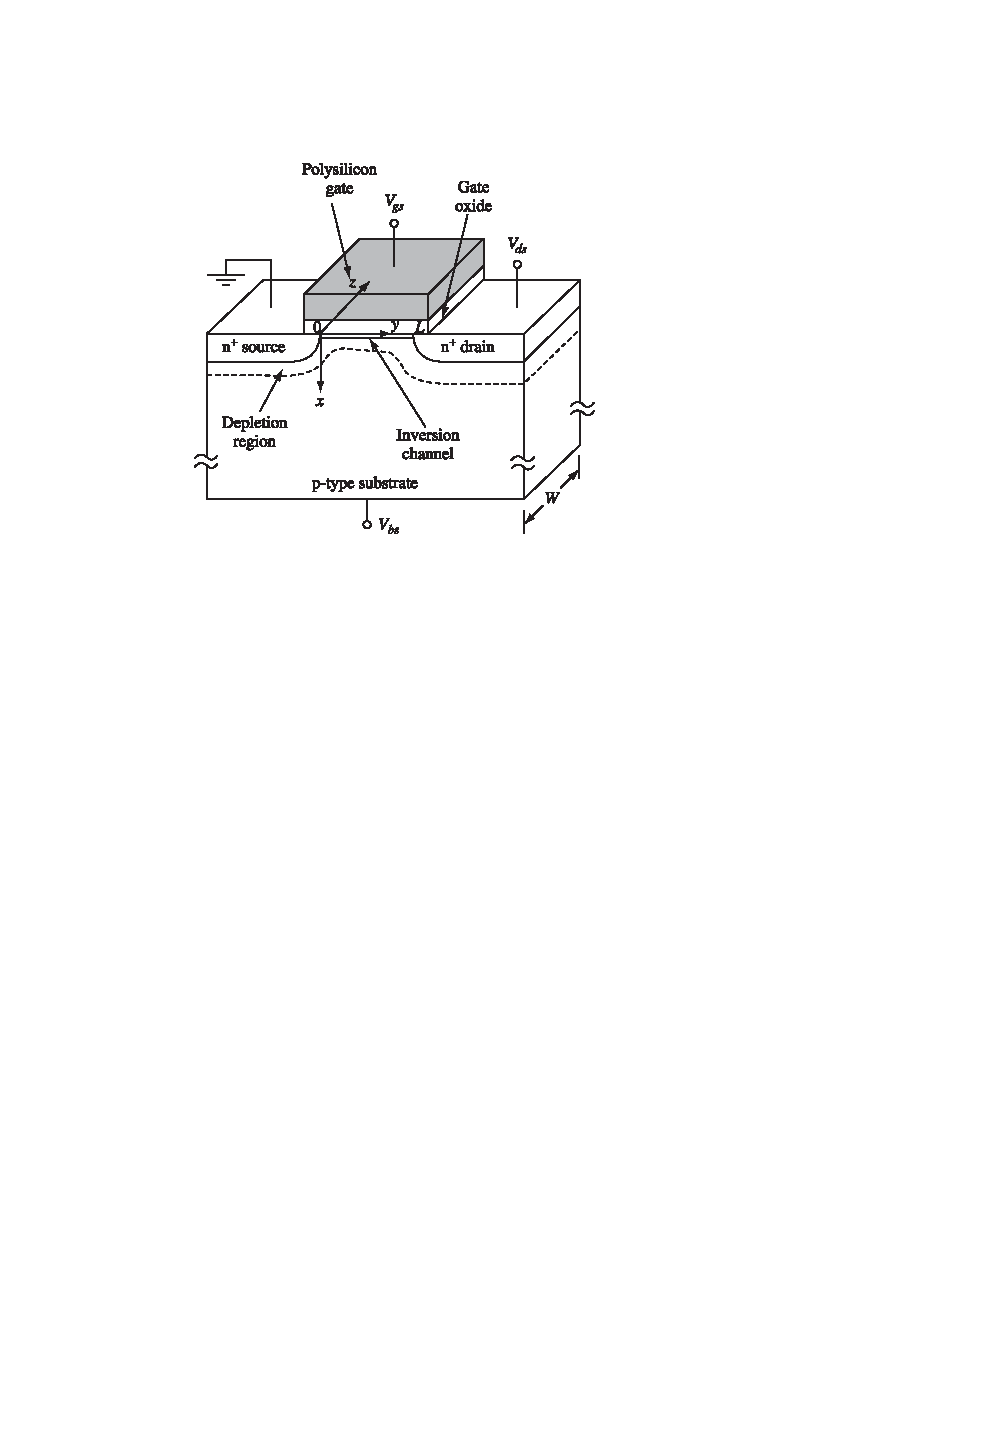
\includegraphics[width=0.5\textwidth]{mosfet_3d.pdf}
    \caption{MOSFET 结构\cite{Modern-VLSI}}
    \label{fig:mosfet_3d}
\end{figure}

%%%
\section{Long-Channel MOSFET I-V Characteristics}

MOSFET 有线性(linear)、饱和(saturation)和截止(cutoff)三种工作状态。以 n-channel 为例,其三种工作状态如图 \ref{fig:mosfet_state} 所示。

\begin{figure}[!htb]
    \centering
    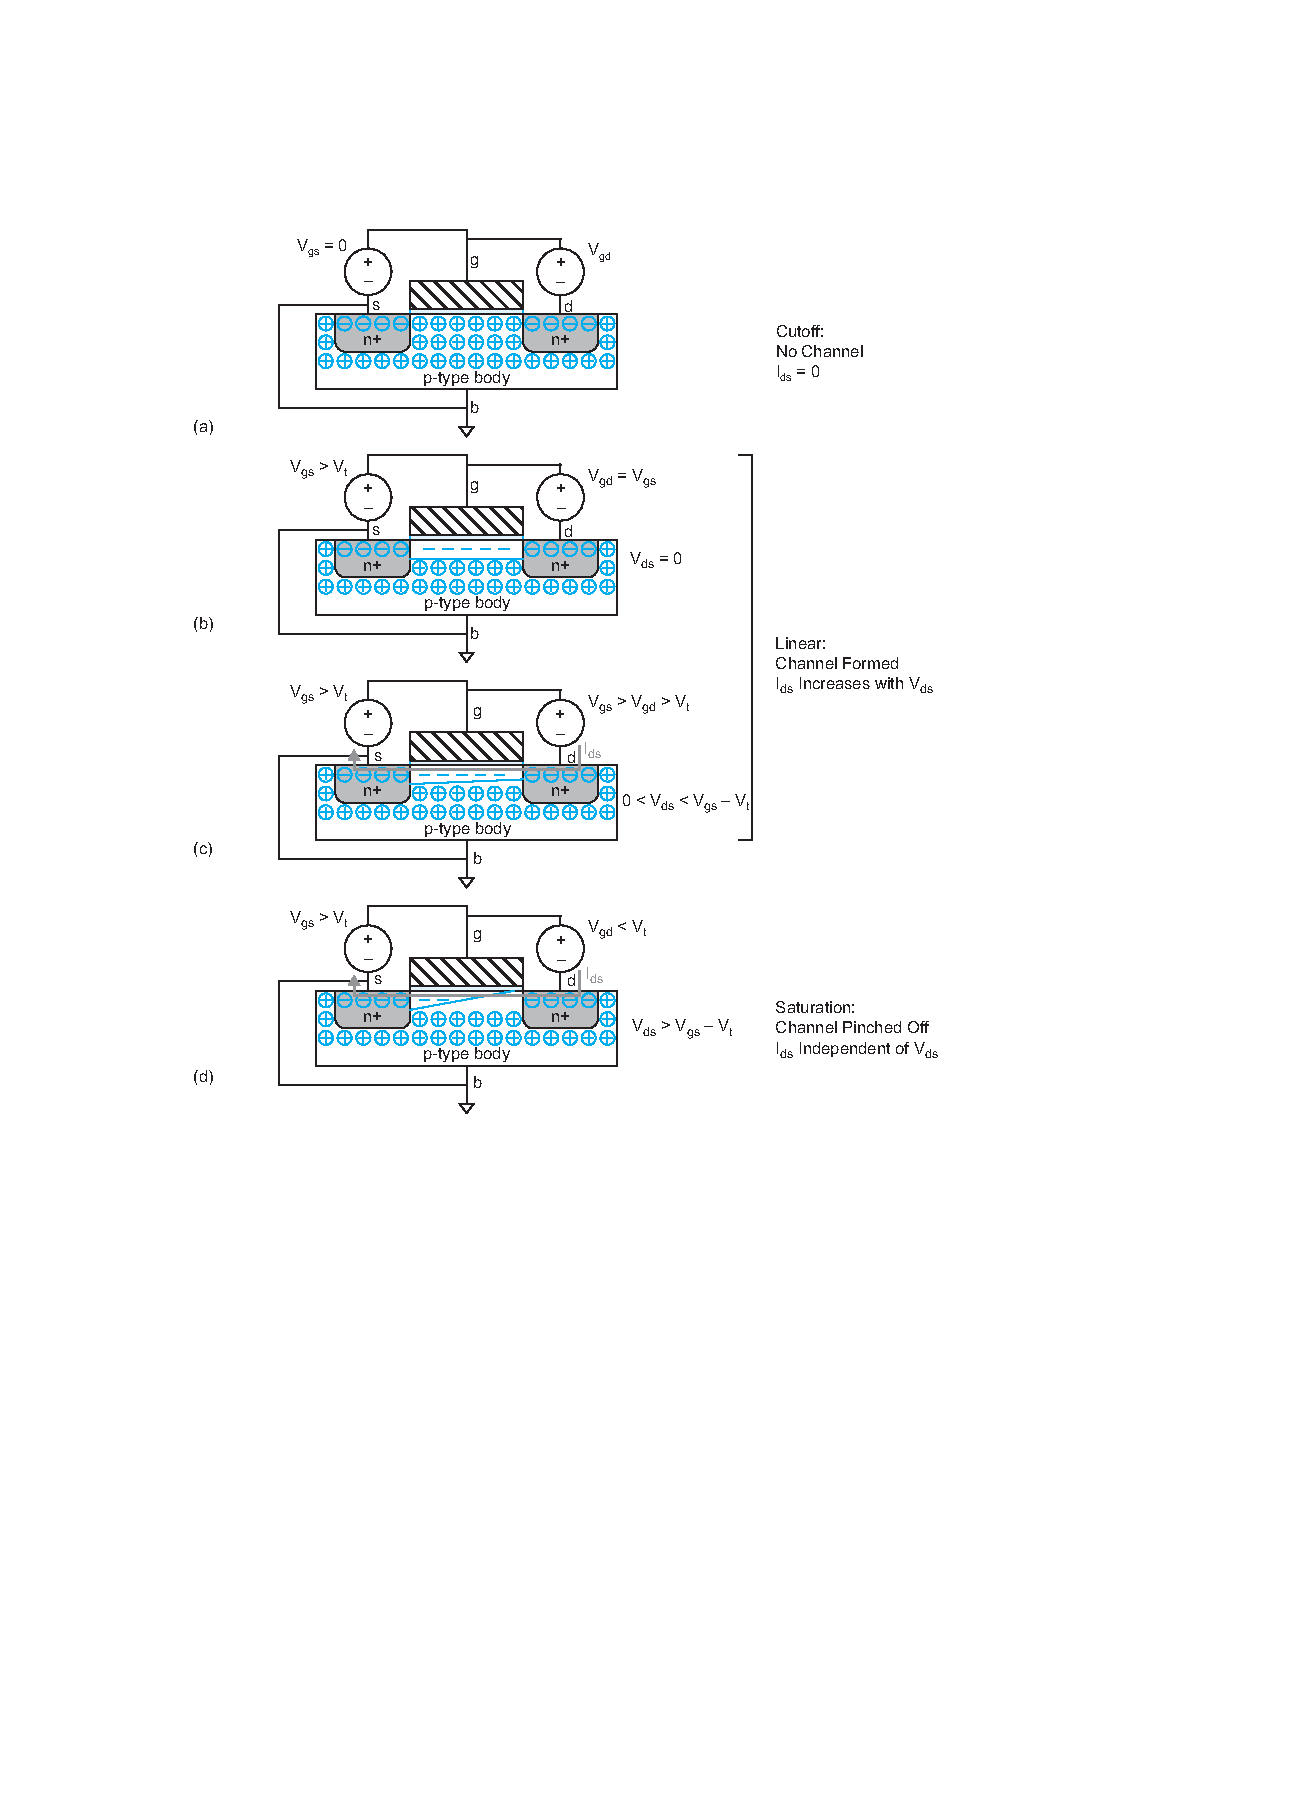
\includegraphics[width=0.7\textwidth]{mosfet_state.pdf}
    \caption{MOSFET 的三种工作状态\cite{CMOS-VLSI}}
    \label{fig:mosfet_state}
\end{figure}

对于 NMOSFET,其 I-V 特性为
\begin{equation}
    I_[D] = 
    \begin{dcases}  % 自动调整上下两行的高度, dfrac fix
        \begin{aligned}
            & 0 && V_[GS] < V_[TH] &&& \text{Cut-off} \\
            & \mu_[n] C_[ox] \frac{W}{L} \left[ (V_[GS] - V_[TH]) V_[DS] - \frac{V_[DS]^2}{2} \right] && V_[GS] \geqslant V_[TH], V_[DS] \leqslant V_[GS] - V_[TH] &&& \text{Linear} \\
            & \frac{1}{2} \mu_[n] C_[ox] \frac{W}{L} (V_[GS] - V_[TH])^2 && V_[GS] \geqslant V_[TH], V_[DS] > V_[GS] - V_[TH] &&& \text{Saturation}
        \end{aligned}
    \end{dcases}
\end{equation}
对于 PMOSFET,其 I-V 特性为
\begin{equation}
    I_[D] = 
    \begin{dcases}  % 自动调整上下两行的高度, dfrac fix
        \begin{aligned}
            & 0 && V_[GS] > V_[TH] &&& \text{Cut-off} \\
            & \mu_[p] C_[ox] \frac{W}{L} \left[ (V_[GS] - V_[TH]) V_[DS] - \frac{V_[DS]^2}{2} \right] && V_[GS] \leqslant V_[TH], V_[DS] \geqslant V_[GS] - V_[TH] &&& \text{Linear} \\
            & \frac{1}{2} \mu_[p] C_[ox] \frac{W}{L} (V_[GS] - V_[TH])^2 && V_[GS] \leqslant V_[TH], V_[DS] < V_[GS] - V_[TH] &&& \text{Saturation}
        \end{aligned}
    \end{dcases}
\end{equation}

%%%
\section{Nonideal I-V Effects}

%%%%
\subsection{Mobility Degradation and Velocity Saturation}

沟道较短的晶体管,也称为短沟器件的行为与长沟器件有所不同,它们不再发生夹断饱和(Pinch-Off Saturation),取而代之的是\textbf{速度饱和(Velocity Saturation)}。

若同时考虑\textbf{速度饱和(Velocity Saturation)}效应,对于 NMOSFET,其 I-V 特性为
\begin{equation}
    I_[D] = 
    \begin{dcases}  % 自动调整上下两行的高度, dfrac fix
        \begin{aligned}
            & 0 && \text{Cut-off} \\
            & \mu_[n] C_[ox] \frac{W}{L} \left[ (V_[GS] - V_[TH]) V_[DS] - \frac{V_[DS]^2}{2} \right] && \text{Linear} \\
            & \frac{1}{2} \mu_[n] C_[ox] \frac{W}{L} (V_[GS] - V_[TH])^2 && \text{Saturation} \\
            & \mu_[n] C_[ox] \frac{W}{L} \left[ (V_[GS] - V_[TH]) V_[DSAT] - \frac{V_[DSAT]^2}{2} \right] && \text{Velocity Saturation}
        \end{aligned}
    \end{dcases}
\end{equation}
各个状态的电压关系为
\begin{equation}
    \begin{aligned}
        & \text{Cut-off:} && V_[GS] < V_[TH] \\
        & \text{Linear:} && V_[GS] \geqslant V_[TH], \min \left(V_[GS] - V_[TH], V_[DS], V_[DSAT]\right) = V_[DS] \\
        & \text{Saturation:} && V_[GS] \geqslant V_[TH], \min \left(V_[GS] - V_[TH], V_[DS], V_[DSAT]\right) = V_[GS] - V_[TH] \\
        & \text{Velocity Saturation:} && V_[GS] \geqslant V_[TH], \min \left(V_[GS] - V_[TH], V_[DS], V_[DSAT]\right) = V_[DSAT]
    \end{aligned}
\end{equation}
而对于 PMOSFET,其 I-V 特性公式与 NMOSFET 相同,但得到的 $I_[D]$ 为负值。
\begin{equation}
    I_[D] = 
    \begin{dcases}  % 自动调整上下两行的高度, dfrac fix
        \begin{aligned}
            & 0 && \text{Cut-off} \\
            & -\mu_[p] C_[ox] \frac{W}{L} \left[ (V_[GS] - V_[TH]) V_[DS] - \frac{V_[DS]^2}{2} \right] && \text{Linear} \\
            & -\frac{1}{2} \mu_[p] C_[ox] \frac{W}{L} (V_[GS] - V_[TH])^2 && \text{Saturation} \\
            & -\mu_[p] C_[ox] \frac{W}{L} \left[ (V_[GS] - V_[TH]) V_[DSAT] - \frac{V_[DSAT]^2}{2} \right] && \text{Velocity Saturation}
        \end{aligned}
    \end{dcases}
\end{equation}
各个状态的电压关系为
\begin{equation}
    \begin{aligned}
        & \text{Cut-off:} && V_[GS] > V_[TH] \\
        & \text{Linear:} && V_[GS] \leqslant V_[TH], \max \left(V_[GS] - V_[TH], V_[DS], V_[DSAT]\right) = V_[DS] \\
        & \text{Saturation:} && V_[GS] \leqslant V_[TH], \max \left(V_[GS] - V_[TH], V_[DS], V_[DSAT]\right) = V_[GS] - V_[TH] \\
        & \text{Velocity Saturation:} && V_[GS] \leqslant V_[TH], \max \left(V_[GS] - V_[TH], V_[DS], V_[DSAT]\right) = V_[DSAT]
    \end{aligned}
\end{equation}

%%%%
\subsection{Channel Length Modulation}
沟道长度调制(Channel Length Modulation)是指沟道长度的变化会导致沟道电阻的变化,从而影响沟道电流。当栅和漏之间的电压差增大时,实际的反型沟道长度逐渐减小。
假设$\Delta L / L$与$V_[DS]$为线性关系,满足
\begin{equation}
    \frac{\Delta L}{L} = \lambda V_[DS]
    \label{eq:channel_length_modulation_coefficient}
\end{equation}
其中 $\lambda$ 即为沟道长度调制系数。在饱和区,电流值需要乘上修正系数 $\left(1 + \lambda V_[DS]\right)$,即
\begin{equation}
    I_[D] = \frac{1}{2} \mu_[n] C_[ox] \frac{W}{L} \left( V_[GS] - V_[TH] \right)^2 \eqnmark[RoyalPurple]{lb}{\left( 1 + \lambda V_[DS] \right)}
\end{equation}
需要注意,沟道长度调制仅在饱和区生效,只有在饱和区才会出现沟道长度的变化$\Delta L$。

类似地,对于 PMOSFET,由于$V_[DS]<0$,考虑沟道长度调制后饱和区的电流为
\begin{equation}
    I_[D] = -\frac{1}{2} \mu_[p] C_[ox] \frac{W}{L} \left( V_[GS] - V_[TH] \right)^2 \eqnmark[RoyalPurple]{lb}{\left( 1 + \lambda V_[DS] \right)}
\end{equation}
注意,根据式 \ref{eq:channel_length_modulation_coefficient},PMOSFET的 $\lambda$ 为负值。

\begin{figure}
    \centering
    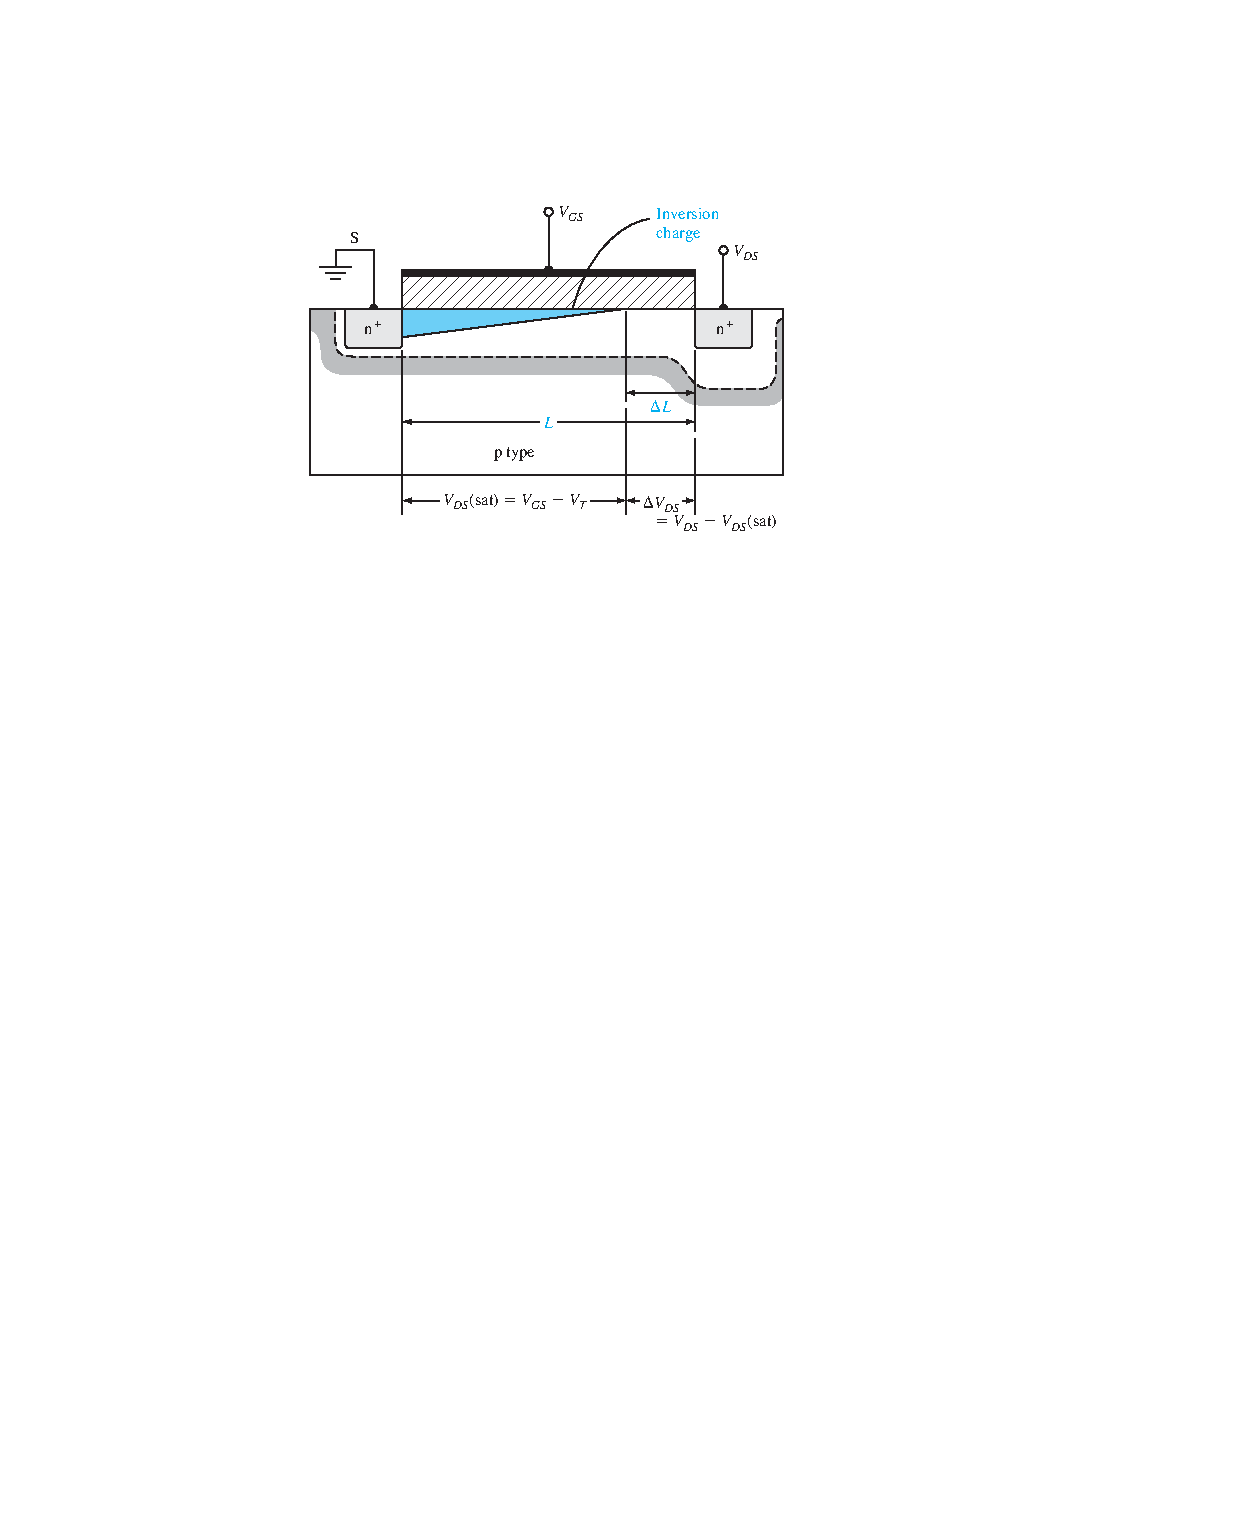
\includegraphics[width=0.7\textwidth]{channel_length_modulation.pdf}
    \caption{沟道长度调制\cite{NeamenSemiconductor}}
    \label{fig:channel_length_modulation}
\end{figure}

%%%%
\subsection{Subthreshold Conduction}

%%%
\subsection{Threshold Voltage Effects}
\subsubsection{Body Effect}
通常情况下,衬底(或称为体)都是与源极相连且接地的,即 $V_[B] = V_[S]$。但是,如果衬底与源极不相连,而是与另一个电压源相连,那么衬底电压 $V_[B]$ 就会影响栅源电压 $V_[GS]$,从而影响晶体管的工作状态。这种现象称为\textbf{体效应(Body Effect)}。

以NMOSFET为例,当衬底存在一个负电压 $V_[B]$ 时,相当于削弱了p型衬底,要达到强反型,栅源电压 $V_[GS]$ 需要增加才能使晶体管进入饱和区,从而阈值电压 $V_[TH]$ 也要相应地增加。

考虑体效应后,NMOSFET 的阈值电压 $V_[TH]$ 为
\begin{equation}
    V_[TH] = V_[TH0] + \gamma \left( \sqrt{|-2 \phi_[F] + V_[SB]|} - \sqrt{|-2 \phi_[F]|} \right)
    \label{eq:threshold_voltage_body_effect}
\end{equation}
其中 $V_[TH0]$ 为 $V_[SB]=0$ 时的阈值电压,$\phi_[F]$ 为费米势,$\gamma$ 为体效应系数,$V_[SB]$ 为源与衬底之间的电压。\\
费米势 $\phi_[F]$ 的定义为费米能级与本征费米能级的能量差,即
\begin{equation}
    \phi_[F]\footnote{在\cite{Analog-CMOS}中,使用的符号为$\varPhi_[F]=-\phi_[F]=E_[Fi]-E_[F]$,存在一个负号的差异。}
    = E_[F] - E_[Fi] 
    = \begin{dcases}
        \begin{aligned}
            & -\dfrac{kT}{q}\ln{\dfrac{N_[A]}{n_[i]}}, && \text{NMOSFET, p型衬底} \\
            & \dfrac{kT}{q}\ln{\dfrac{N_[D]}{n_[i]}}, && \text{PMOSFET, n型衬底}
        \end{aligned}
    \end{dcases}
\end{equation}
体效应系数 $\gamma$ 反映了衬底电压对阈值电压的影响程度,其值与衬底掺杂浓度 $N_[A]$ 或 $N_[D]$ 有关,计算公式为
\begin{equation}
    \gamma =
    \begin{dcases}
        \begin{aligned}
            & \dfrac{\sqrt{2q\varepsilon_[Si]N_[A]}}{C_[ox]}, && \text{NMOSFET, p型衬底} \\
            & -\dfrac{\sqrt{2q\varepsilon_[Si]N_[D]}}{C_[ox]}, && \text{PMOSFET, n型衬底}
        \end{aligned}
    \end{dcases}
\end{equation}
NMOSFET 的阈值电压 $V_[TH]$ 受 $V_[BS]$(不是$V_[SB]$) 影响的情况如图 \ref{fig:threshold_voltage_body_effect} 所示。
\begin{figure}[!htb]
    \centering
    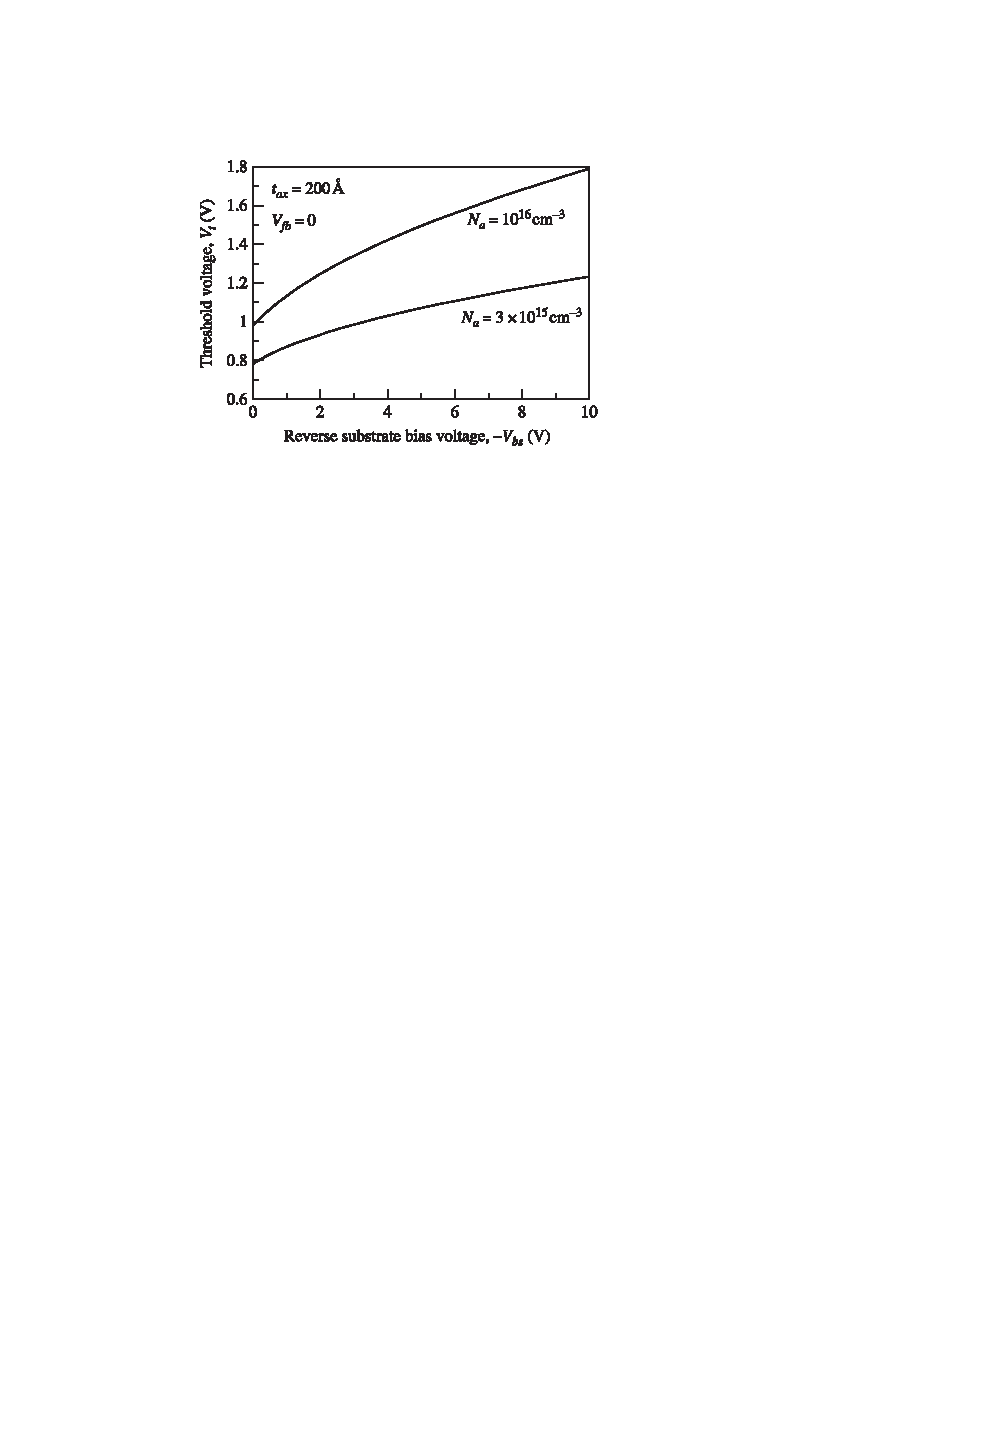
\includegraphics[width=0.6\textwidth]{threshold_voltage_body_effect.pdf}
    \caption{NMOSFET 的体效应\cite{Modern-VLSI}}
    \label{fig:threshold_voltage_body_effect}
\end{figure}
如果对符号感到困惑,请注意
\begin{itemize}
    \item 对于 NMOSFET,费米势 $\phi_[F]$ 为负,衬底偏置 $V_[SB]$ 通常为正,$V_[TH]$ 也为正,且 $\Delta V_[TH] > 0$。
    \item 对于 PMOSFET,费米势 $\phi_[F]$ 为正,衬底偏置 $V_[SB]$ 通常为负,$V_[TH]$ 也为负,且 $\Delta V_[TH] < 0$。
\end{itemize}

\subsubsection{Drain-Induced Barrier Lowering}

\subsubsection{Short Channel Effect}

%%%
\section{MOSFET I-V Characteristics Summary}

为了简化公式,引入工艺因子$k$(Gain Factor)和工艺跨导$k'$(Transconductance)的概念。\\
工艺因子 $k$ 为
\begin{equation}
    \begin{aligned}
        k_[n] &= \mu_[n] C_[ox] \frac{W}{L} \\
        k_[p] &= -\mu_[p] C_[ox] \frac{W}{L}
    \end{aligned}
\end{equation}
工艺跨导 $k'$ 为
\begin{equation}
    \begin{aligned}
        k'_[n] &= \mu_[n] C_[ox] \\
        k'_[p] &= -\mu_[p] C_[ox]
    \end{aligned}
\end{equation}

这样,NMOSFET 的 I-V 特性为(非截止区)
\begin{equation}
    I_[D] = k_[n] \left[ (V_[GS] - V_[TH]) V_[min] - \frac{V_[min]^2}{2} \right] \left(1 + \lambda V_[DS]\right)
\end{equation}
其中 $V_[min] = \min \left(V_[GS] - V_[TH], V_[DS], V_[DSAT]\right)$。\\
PMOSFET 的 I-V 特性为
\begin{equation}
    I_[D] = k_[p] \left[ (V_[GS] - V_[TH]) V_[max] - \frac{V_[max]^2}{2} \right] \left(1 + \lambda V_[DS]\right)
\end{equation}
其中 $V_[max] = \max \left(V_[GS] - V_[TH], V_[DS], V_[DSAT]\right)$。

\begin{figure}[!hbt]
    \centering
    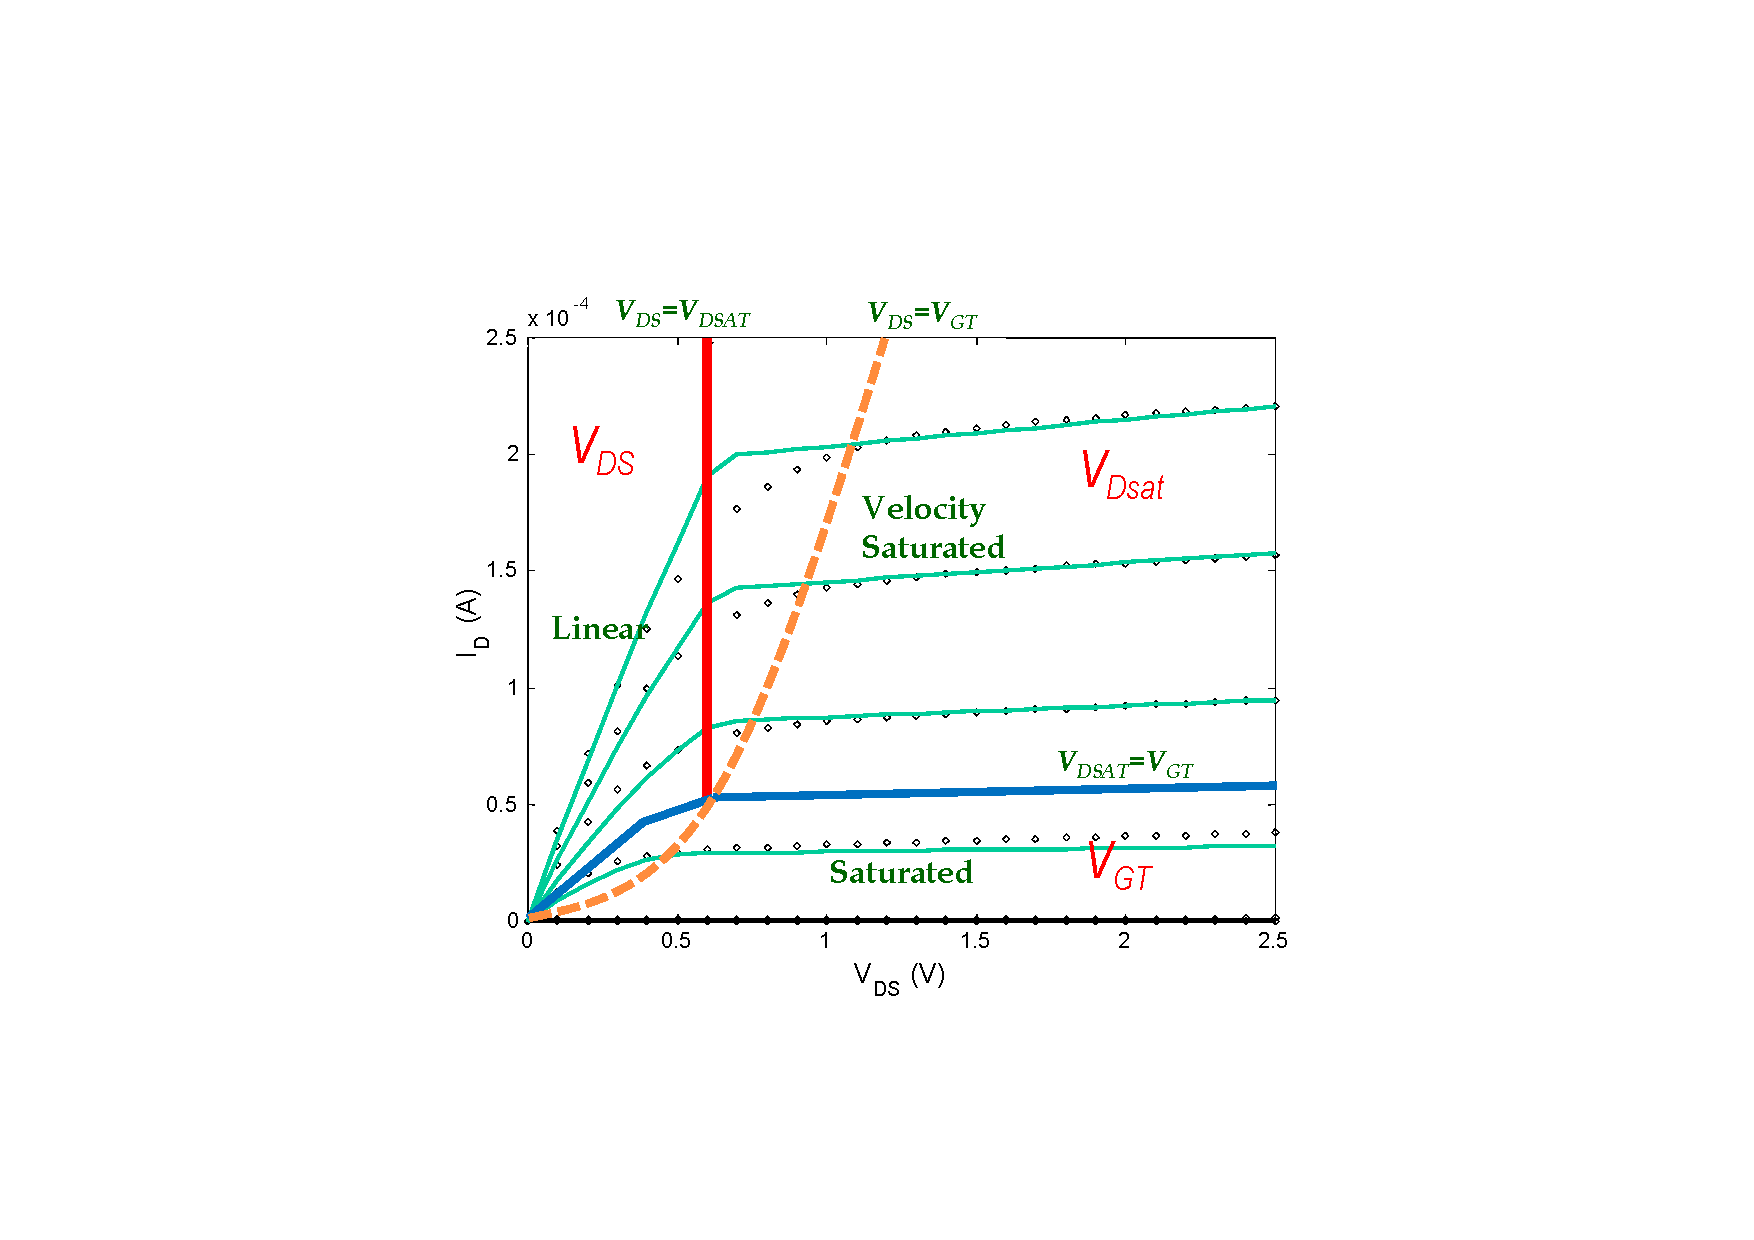
\includegraphics[width=0.6\textwidth]{nmos_iv_regions.pdf}
    \caption{NMOSFET 的工作状态}
    \label{fig:nmos_iv_regions}
\end{figure}

%%%
\section{MOSFET C-V Characteristics}

MOSFET 的电容可以概括为栅、漏、源、体四个 terminal 之间的电容,如图 \ref{fig:mosfet_capacitance} 所示。

\begin{figure}[!htb]
    \centering
    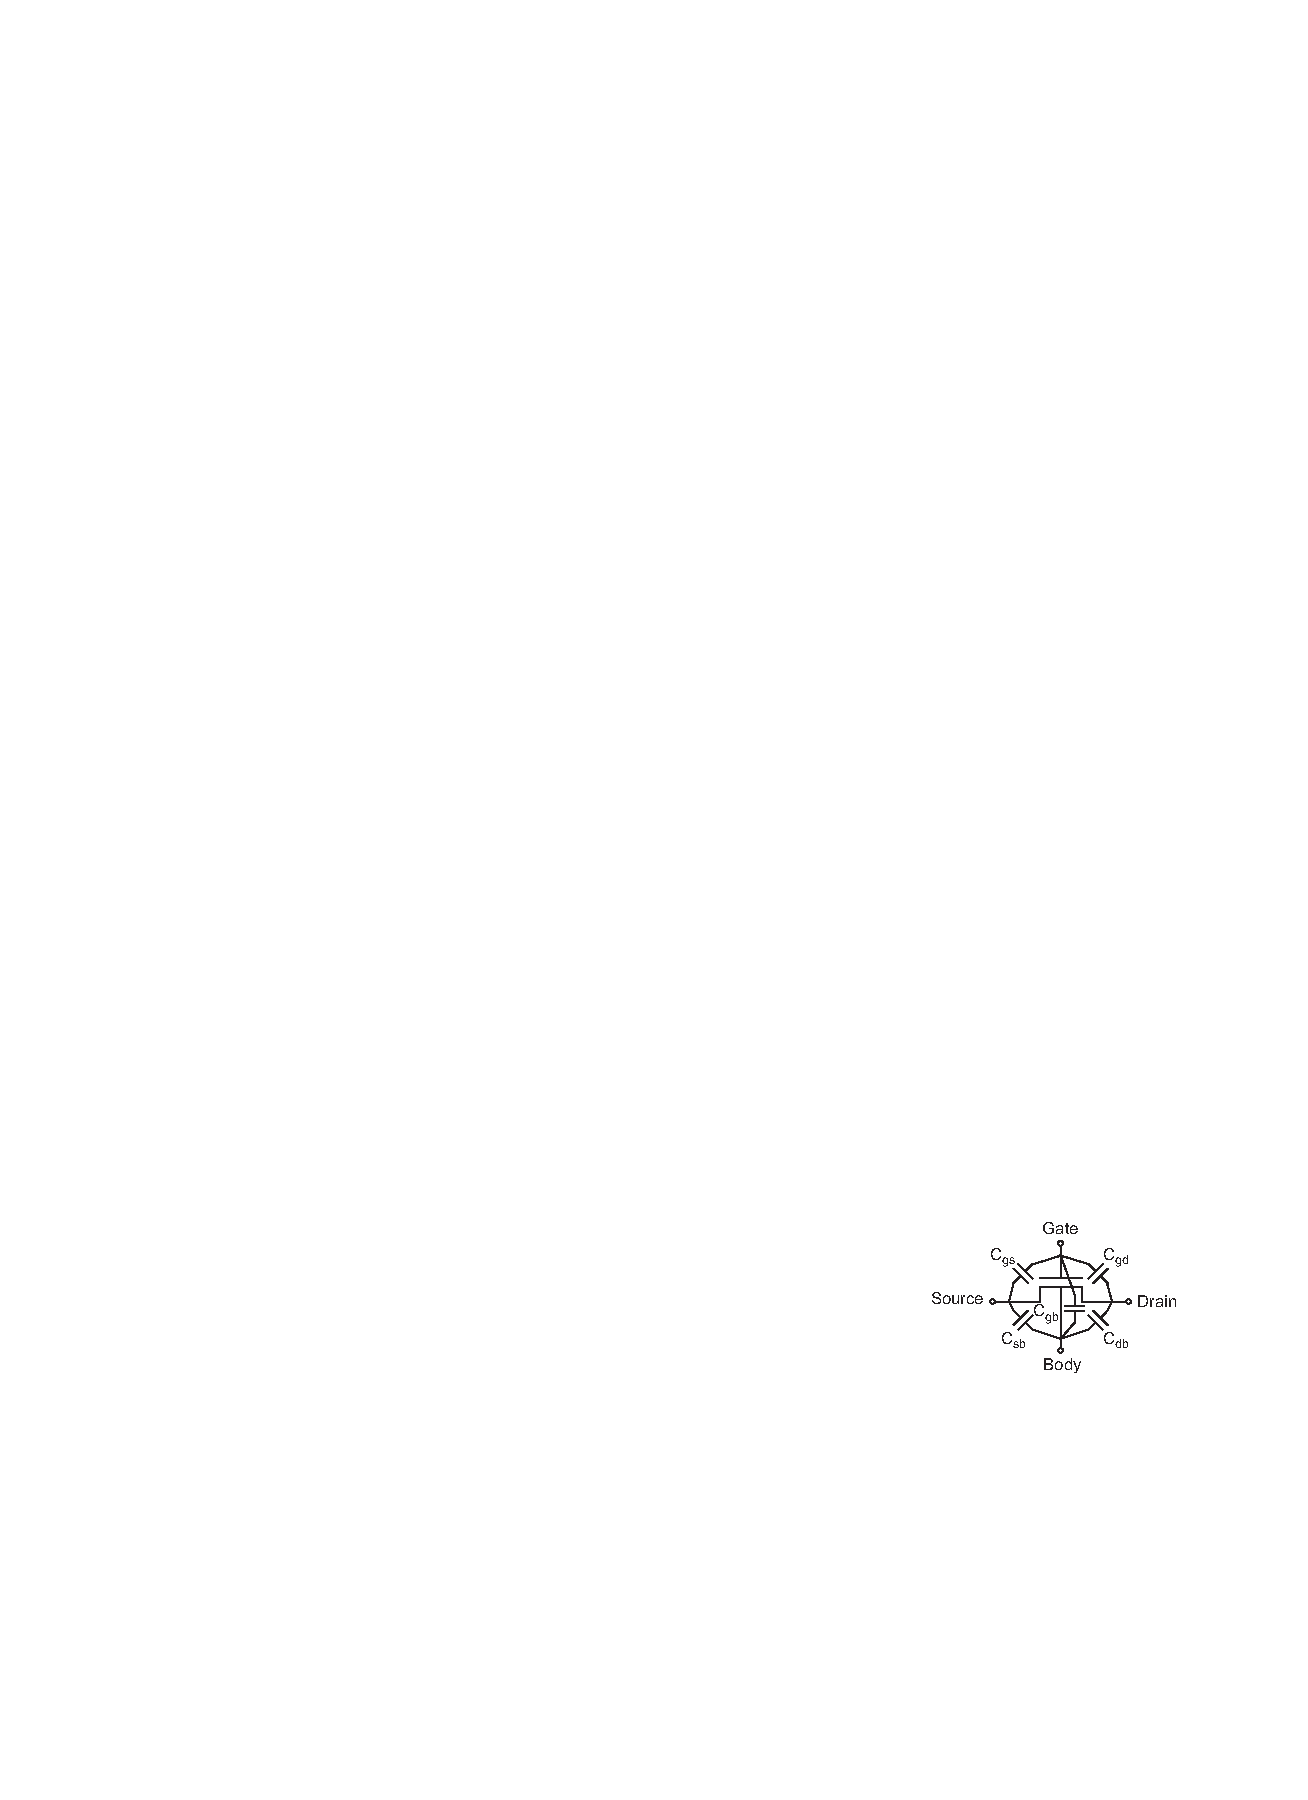
\includegraphics[width=0.5\textwidth]{MOS_Capacitance.pdf}
    \caption{MOSFET 的电容\cite{CMOS-VLSI}}
    \label{fig:mosfet_capacitance}
\end{figure}

电容的来源可以分为以下三部分:
\begin{itemize}
    \item \textbf{结构电容(MOS structure capacitances)}:结构电容是由于 MOS 结构的特性而产生的电容。结构电容的大小与 MOS 结构的面积、厚度、介电常数有关。
    \begin{itemize}
        \item 覆盖电容(Overlap Capacitance):$C_[overlap] = C_[GSO] + C_[GDO]$。覆盖电容是由源和漏在氧化层下延展的横向扩散所引起的栅和源漏间的寄生电容。
    \end{itemize}
    \item \textbf{栅至沟道的电容(Gate-to-channel Capacitance)}:$C_[GC] = C_[GCB] + C_[GCS] + C_[GCD]$。沟道电容取决于晶体管的工作区间,产生晶体管工作所需的沟道电荷。
    \begin{itemize}
        \item 栅体沟道电容(Gate-Body Channel Capacitance):$C_[GCB]$。
        \item 栅源沟道电容(Gate-Source Channel Capacitance):$C_[GCS]$。
        \item 栅漏沟道电容(Gate-Drain Channel Capacitance):$C_[GCD]$。
    \end{itemize}
    \item \textbf{扩散电容/结电容(Juction/Diffusion Capacitance)}:$C_[diff] = C_[Sdiff] + C_[Ddiff]$。扩散电容/结电容是扩散区处于反向偏置的源体、漏体间的pn结引起的电容。
    \begin{itemize}
        \item 源扩散电容(Source Diffusion Capacitance):$C_[Sdiff]$。
        \item 漏扩散电容(Drain Diffusion Capacitance):$C_[Ddiff]$。
    \end{itemize}
\end{itemize}

这样,栅电容 $C_[GS]$, $C_[GB]$, $C_[GD]$ 分别可以表示为
\begin{equation}
    \begin{aligned}
        C_[GS] &= C_[GCS] + C_[GSO] \\
        C_[GB] &= C_[GCB] \\
        C_[GD] &= C_[GCD] + C_[GDO]
    \end{aligned}
\end{equation}
结电容 $C_[SB]$, $C_[DB]$ 分别可以表示为
\begin{equation}
    \begin{aligned}
        C_[SB] &= C_[Sdiff] \\
        C_[DB] &= C_[Ddiff]
    \end{aligned}
\end{equation}

电容相关的符号如表 \ref{tab:mosfet-capacitance-symbols} 所示。
\begin{table}[!htb]
    \centering
    \caption{MOSFET 电容符号表}
    \label{tab:mosfet-capacitance-symbols}
    \scalebox{0.82}{ % 缩放表格
    \begin{NiceTabular}{cccc}
        \Xhline{1pt}
        \textbf{Symbol} & \textbf{Meaning} & \textbf{Unit} & \textbf{Polarity} \\ \hline
        $C_[GS]$ & 栅源电容(Gate-Source capacitance) & $\unit{\farad}$ & + \\
        $C_[GB]$ & 栅体电容(Gate-Body capacitance) & $\unit{\farad}$ & + \\
        $C_[GD]$ & 栅漏电容(Gate-Drain capacitance) & $\unit{\farad}$ & + \\
        $C_[SB]$ & 源体电容(Source-Body capacitance) & $\unit{\farad}$ & + \\
        $C_[DB]$ & 漏体电容(Drain-Body capacitance) & $\unit{\farad}$ & + \\
        $C_[ox]$ & 单位面积栅氧电容(Gate Oxide Capacitance per unit area) & $\unit{\farad \per \meter \squared}$ & + \\
        $C_[overlap]$ & 总覆盖电容(Overlap capacitance) & $\unit{\farad}$ & + \\
        $C_[GSO]$ & 栅源间覆盖电容(Gate-Source Overlap capacitance) & $\unit{\farad}$ & + \\
        $C_[GDO]$ & 栅漏间覆盖电容(Gate-Drain Overlap capacitance) & $\unit{\farad}$ & + \\
        $C_[o]$ & 单位晶体管宽度覆盖电容(Overlap capacitance per unit transistor width) & $\unit{\farad \per \meter}$ & + \\
        $x_[d]$ & 横向扩散距离(Lateral diffusion distance) & $\unit{\meter}$ & + \\
        $C_[GC]$ & 栅沟道电容(Gate-Channel capacitance) & $\unit{\farad}$ & + \\
        $C_[GCB]$ & 栅体沟道电容(Gate-Body Channel capacitance) & $\unit{\farad}$ & + \\
        $C_[GCS]$ & 栅源沟道电容(Gate-Source Channel capacitance) & $\unit{\farad}$ & + \\
        $C_[GCD]$ & 栅漏沟道电容(Gate-Drain Channel capacitance) & $\unit{\farad}$ & + \\
        $C_[Sdiff]$ & 源扩散电容(Source Diffusion Capacitance) & $\unit{\farad}$ & + \\
        $C_[Ddiff]$ & 漏扩散电容(Drain Diffusion Capacitance) & $\unit{\farad}$ & + \\
        $C_[bottom]$ & 底板电容(Bottom-plate capacitance) & $\unit{\farad}$ & + \\
        $C_[sw]$ & 侧壁电容(SideWall capacitance) & $\unit{\farad}$ & + \\
        $C_[J]$ & 零偏单位面积底板电容(Zero-bias bottom-plate capacitance per unit area) & $\unit{\farad \per \meter \squared}$ & + \\
        $C_[JSW]$ & 零偏单位面积侧壁电容(Zero-bias side-wall capacitance per unit area) & $\unit{\farad \per \meter \squared}$ & + \\
        $C_[jbs]$ & 体源单位面积结电容(Body-to-Source bottom-plate junction cap per unit area) & $\unit{\farad \per \meter \squared}$ & + \\
        $C_[jbd]$ & 体漏单位面积结电容(Body-to-Drain bottom-plate junction cap per unit area) & $\unit{\farad \per \meter \squared}$ & + \\
        AS & 源区底板面积(Area of bottom plate in Source region) & $\unit{\meter \squared}$ & + \\
        AD & 漏区底板面积(Area of bottom plate in Drain region) & $\unit{\meter \squared}$ & + \\
        $\psi_0$ & 内建电势(Built-in potential) & $\unit{\volt}$ & + \\
        $C_[jbssw]$ & 体源侧壁单位面积结电容(Body-to-Source side-wall junction cap per unit area) & $\unit{\farad \per \meter \squared}$ & + \\
        $C_[jbdsw]$ & 体漏侧壁单位面积结电容(Body-to-Drain side-wall junction cap per unit area) & $\unit{\farad \per \meter \squared}$ & + \\
        $C_[jbsswg]$ & 单位宽度的面向沟道源侧壁电容(Source beside Gate side-wall junction cap per unit perimeter) & $\unit{\farad \per \meter}$ & + \\
        $C_[jbdswg]$ & 单位宽度的面向沟道漏侧壁电容(Drain beside Gate side-wall junction cap per unit perimeter) & $\unit{\farad \per \meter}$ & + \\
        $M_[J]$ & 底板结电容结缓变系数(Bottom-plate junction capacitance grading coefficient) & 1 & + \\
        $M_[JSW]$ & 侧壁结电容结缓变系数(Side-wall junction capacitance grading coefficient) & 1 & + \\
        $M_[JSWG]$ & 沟道侧壁结电容结缓变系数(Gate side-wall junction capacitance grading coefficient) & 1 & + \\
        \Xhline{1pt}
    \end{NiceTabular}
    }
\end{table}


%%%%
\subsection{Gate Capacitance}
栅电容可以进一步分为两部分:\textbf{覆盖电容$C_[overlap]$}和\textbf{沟道电容$C_[GC]$}。
\subsubsection{Structure Capacitance — Overlap Capacitance}
当通过扩散形成源区和漏区时,理想中,源和漏的扩散应当恰好终止在栅氧的边界上,但是,实际情况是,源和漏的边界都会往栅氧下延伸$x_[d]$的距离,这被称为横向扩散,这就导致了栅氧覆盖了一定面积的源区和漏区,从而形成了栅和源漏间的\textbf{覆盖电容(Overlap Capacitance)},如图 \ref{fig:overlap_capacitance} 所示。
\begin{figure}[!htb]
    \centering
    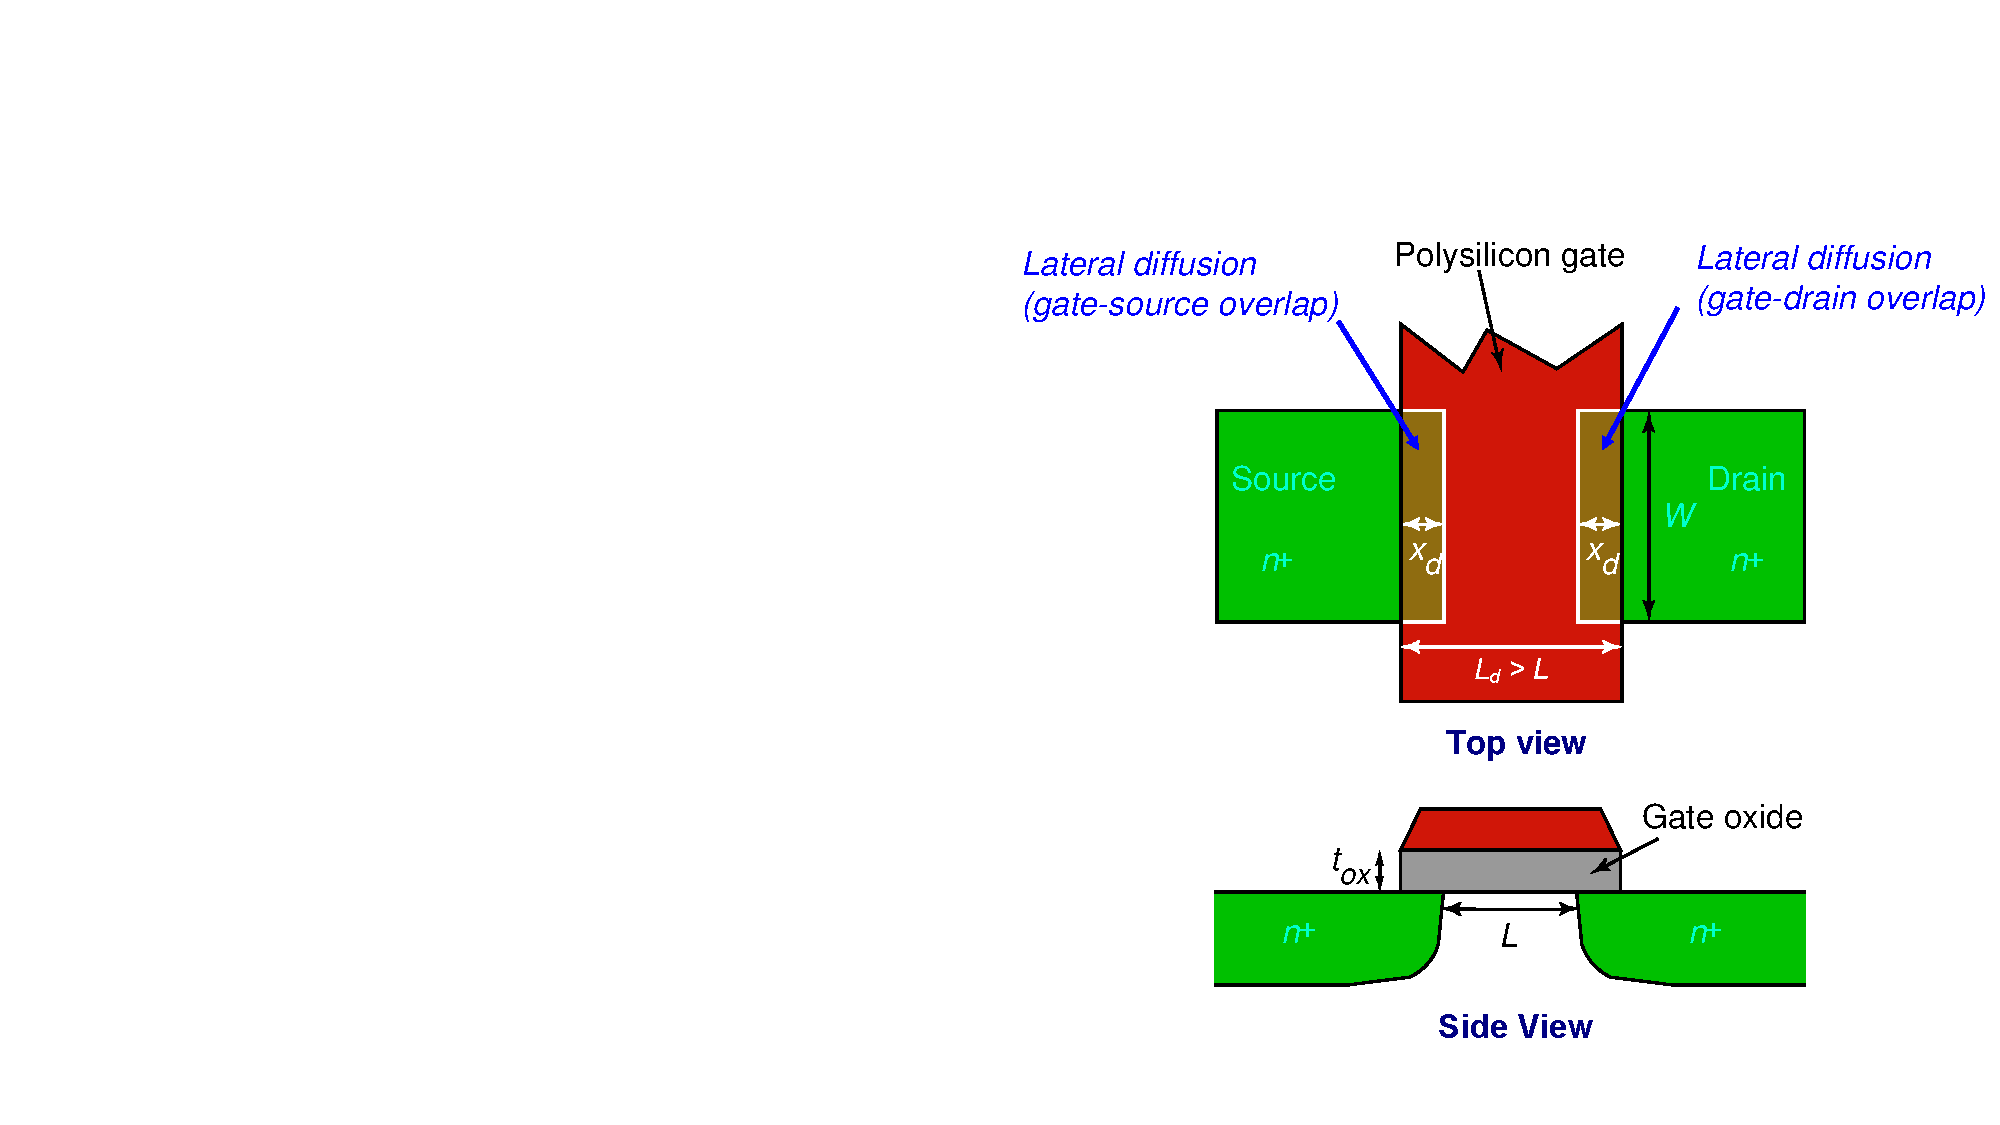
\includegraphics[width=0.5\textwidth]{MOS_overlap.pdf}
    \caption{覆盖电容}
    \label{fig:overlap_capacitance}
\end{figure}

假设两侧的横向扩散距离相同,即$x_[d] = x_[dS] = x_[dD]$,则覆盖电容为
\begin{equation}
    \begin{aligned}
        C_[GSO] &= C_[GDO] = C_[ox] x_[d] W = C_[o] W \\
        C_[overlap] &= C_[GSO] + C_[GDO] = 2 C_[ox] x_[d] W = 2 C_[o] W \\
    \end{aligned}\label{eq:overlap-capacitance}
\end{equation}
其中 $C_[ox]$ = ${\varepsilon_[ox]}$ / ${t_[ox]}$。

\subsubsection{Gate-to-Channel Capacitance}
沟道电容的计算可以使用一个简单的线性化模型,如表 \ref{tab:gate2channel-model} 所示。
\begin{table}[h!tb]
    \centering
    \caption{沟道电容模型}
    \label{tab:gate2channel-model}
    \begin{NiceTabular}{c|cccc}
        \Xhline{1pt}
        Operation Region & $C_[GCB]$ & $C_[GCS]$ & $C_[GCD]$ & $C_[GC] = C_[GCB] + C_[GCS] + C_[GCD]$ \\ \hline
        cut-off & $C_[ox]WL$ & 0 & 0 & $C_[ox]WL$ \\
        linear & 0 & $C_[ox]WL/2$ & $C_[ox]WL/2$ & $C_[ox]WL$ \\
        saturation & 0 & $(2/3)C_[ox]WL$ & 0 & $(2/3)C_[ox]WL$ \\
        \Xhline{1pt}
    \end{NiceTabular}
\end{table}

三种工作状态下的沟道电容如图 \ref{fig:gate2channel-capacitance} 所示。
\begin{figure}[!htb]
    \centering
    \begin{subfigure}[b]{0.4\textwidth}
        \centering
        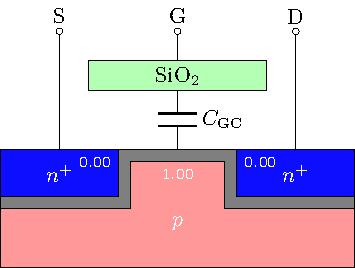
\includegraphics[width=6cm]{C_GC_cutoff.pdf}
        \caption{截止区}
    \end{subfigure}
    \begin{subfigure}[b]{0.4\linewidth}
        \centering
        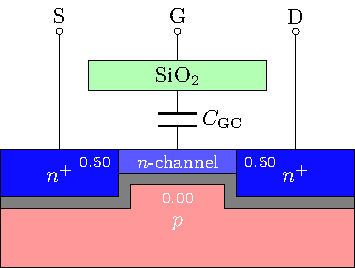
\includegraphics[width=6cm]{C_GC_linear.pdf}
        \caption{线性区}
    \end{subfigure}
    \begin{subfigure}[b]{\linewidth}
        \centering
        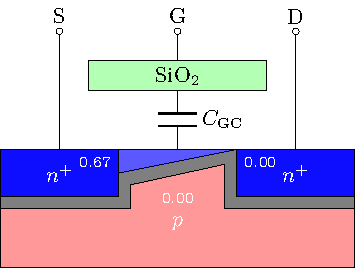
\includegraphics[width=6cm]{C_GC_saturation.pdf}
        \caption{饱和区}
    \end{subfigure}
    \caption{三种工作状态下的沟道电容\cite{DigitalIC_lyx}}
    \label{fig:gate2channel-capacitance}
\end{figure}

\subsubsection{Gate Capacitance Summary}
式 \ref{eq:overlap-capacitance} 指出覆盖电容$C_[overlap]$的值为$2 C_[o] W$,而表 \ref{tab:gate2channel-model} 给出了沟道电容$C_[GC]$的值,因此,栅电容$C_[G]$的值可用表 \ref{tab:gate-capacitance-summary} 总结。
\begin{table}[!htb]
    \centering
    \caption{栅电容总结}
    \label{tab:gate-capacitance-summary}
    \begin{NiceTabular}{c|cccc}
        \Xhline{1pt}
        \textbf{Region} & $C_[GB] = C_[GCB]$ & $C_[GS] = C_[GSO] + C_[GCS]$ & $C_[GD] = C_[GDO] + C_[GCD]$ & $C_[G] = C_[GS] + C_[GB] + C_[GD]$ \\ \hline
        cut-off & $C_[ox]WL$ & $C_[o]W$ & $C_[o]W$ & $C_[ox]WL + 2C_[o]W$ \\
        linear & 0 & $C_[o]W + C_[ox]WL/2$ & $C_[o]W + C_[ox]WL/2$ & $C_[ox]WL + 2C_[o]W$ \\
        saturation & 0 & $C_[o]W + (2/3)C_[ox]WL/2$ & $C_[o]W$ & $(2/3)C_[ox]WL + 2C_[o]W$ \\
        \Xhline{1pt}
    \end{NiceTabular}
\end{table}

\subsection{Junction/Diffusion Capacitance}
扩散电容/结电容是扩散区处于反向偏置的源体、漏体间的pn结引起的电容。可分为源扩散电容$C_[SB]/C_[Sdiff]$和漏扩散电容$C_[DB]/C_[Ddiff]$两部分。如图 \ref{fig:diffusion-capacitance} 所示。
\begin{figure}[!htb]
    \centering
    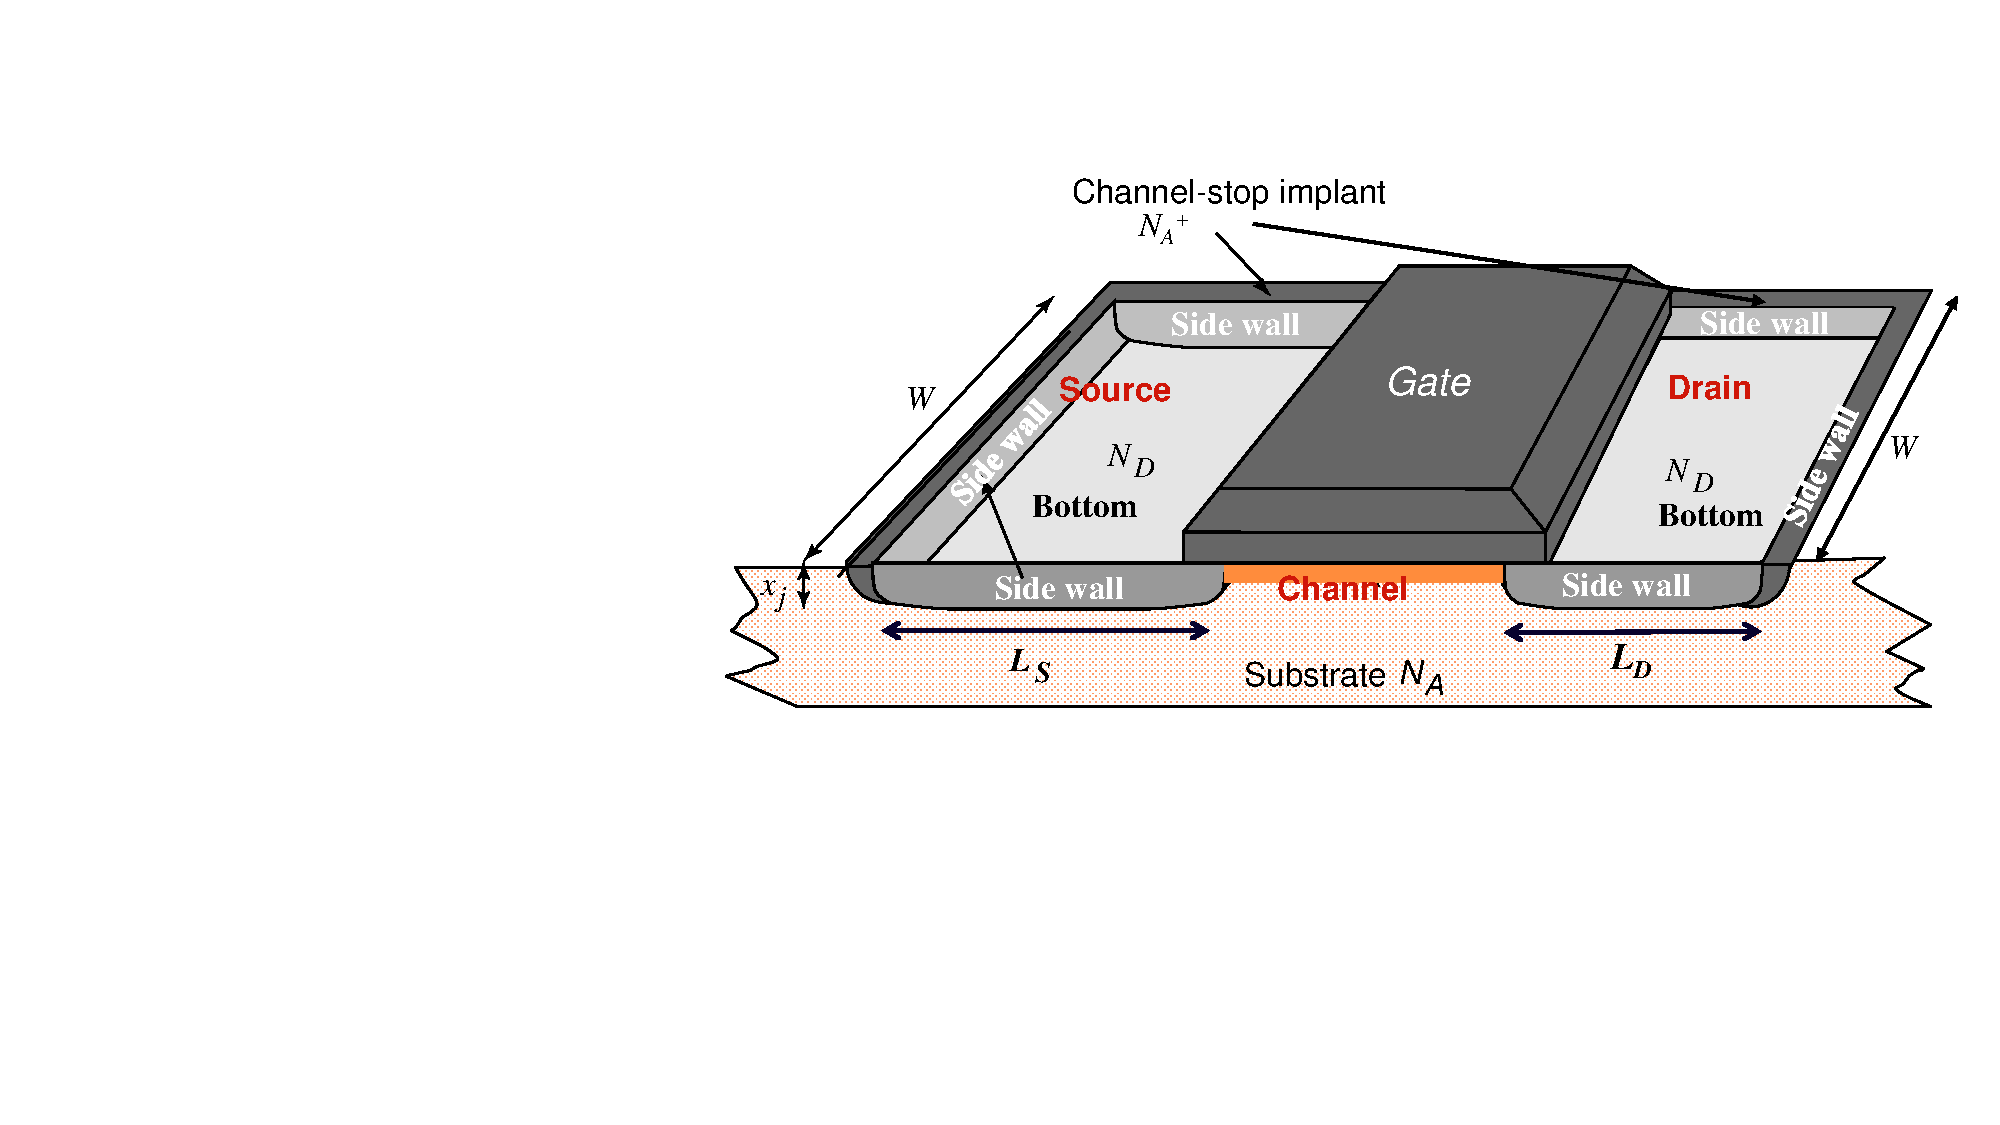
\includegraphics[width=0.7\textwidth]{MOS_diffusion_cap.pdf}
    \caption{扩散电容/结电容}
    \label{fig:diffusion-capacitance}
\end{figure}

扩散电容的计算分为两部分,\textbf{底板电容$C_[bottom]$}(Bottom Plate Capacitance)和\textbf{侧壁电容$C_[sw]$(Side Wall Capacitance)}。

底板电容是源和漏底部与衬底之间的结电容,其计算公式为
\begin{equation}
    \begin{aligned}
        C_[bottom,SB] &= C_[jbs]\cdot\mathrm{AS} \\
        C_[bottom,DB] &= C_[jbd]\cdot\mathrm{AD}
    \end{aligned}
\end{equation}
其中$\mathrm{AS} = L_[S]W$是源区底板的面积,$\mathrm{AD} = L_[D]W$是漏区底板的面积(A表示Area)。而$C_[jbs]$是单位面积的体到源结电容,$C_[jbd]$是单位面积的体到漏结电容。
在SPICE模型中,它们的值由式 \ref{eq:bottom-plate-capacitance} 给出
\begin{equation}
    \begin{aligned}
        C_[jbs] &= C_[J] \left(1 + \dfrac{V_[SB]}{\psi_0}\right)^{-M_[J]} \\
        C_[jbd] &= C_[J] \left(1 + \dfrac{V_[DB]}{\psi_0}\right)^{-M_[J]}
    \end{aligned}
    \label{eq:bottom-plate-capacitance}
\end{equation}
其中$C_[J]$是零偏时单位面积的底板电容,$\psi_[0]$是体-源/漏结的内建电势\footnote{$\psi_{0} = \dfrac{kT}{q}\ln\left(\dfrac{N_[D]N_[A]}{n_[i]^2}\right)$},$M_[J]$是结电容的调制系数(约0.5)。

侧壁电容是源和漏侧壁与衬底之间的结电容。由于工艺原因,沿非导电沟道的侧壁电容往往很小,而面向沟道的侧壁电容则更大。因此,侧壁电容的计算公式为
\vspace{1em}
\begin{equation}
    \begin{aligned}
        C_[sw,SB] &= \eqnmarkbox[blue]{node1}{C_[jbssw] \cdot \mathrm{PS}} + \eqnmarkbox[red]{node2}{C_[jbsswg] \cdot W} \\
        C_[sw,DB] &= C_[jbdsw] \cdot \mathrm{PD} + C_[jbdswg] \cdot W
    \end{aligned}
    \annotate[yshift=0.5em]{left}{node1}{非导电沟道的侧壁电容}
    \annotate[yshift=0.5em]{right}{node2}{面向沟道的侧壁电容}
\end{equation}
其中$\mathrm{PS} = 2L_[S] + W$是源区侧壁的周长,$\mathrm{PD} = 2L_[D] + W$是漏区侧壁的周长(P表示Perimeter)。而$C_[jbssw]$是单位周长的源侧壁电容,$C_[jbdsw]$是单位周长的漏侧壁电容,$C_[jbsswg]$是单位宽度的面向沟道源侧壁电容,$C_[jbdswg]$是单位宽度的面向沟道漏侧壁电容。
在SPICE模型中,它们的值由式 \ref{eq:side-wall-capacitance} 给出
\begin{equation}
    \begin{aligned}
        C_[jbssw] &= C_[JSW] \left(1 + \dfrac{V_[SB]}{\psi_0}\right)^{-M_[JSW]} \\
        C_[jbdsw] &= C_[JSW] \left(1 + \dfrac{V_[DB]}{\psi_0}\right)^{-M_[JSW]} \\
        C_[jbsswg] &= C_[JSW] \left(1 + \dfrac{V_[SB]}{\psi_0}\right)^{-M_[JSWG]} \\
        C_[jbdswg] &= C_[JSW] \left(1 + \dfrac{V_[DB]}{\psi_0}\right)^{-M_[JSWG]}
    \end{aligned}
    \label{eq:side-wall-capacitance}
\end{equation}
其中$C_[JSW]$是零偏时单位周长的侧壁电容,$M_[JSW]$是侧壁电容的调制系数(约0.33),$M_[JSWG]$是面向沟道侧壁电容的调制系数(约0.33)。

总结以上内容,扩散电容/结电容的计算公式为
\begin{equation}
    \begin{aligned}
        C_[SB] &= C_[bottom,SB] + C_[sw,SB] = C_[jbs]\cdot\mathrm{AS} + C_[jbssw] \cdot \mathrm{PS} + C_[jbsswg] \cdot W \\
        C_[DB] &= C_[bottom,DB] + C_[sw,DB] = C_[jbd]\cdot\mathrm{AD} + C_[jbdsw] \cdot \mathrm{PD} + C_[jbdswg] \cdot W
    \end{aligned}
\end{equation}

%%%
\section{MOSFET Small Signal Model}

小信号模型是指在某一工作点附近,将非线性的电路元件用线性的电路元件来近似表示的模型,是一种一阶的近似。
在许多模拟电路中,MOSFETs 工作在饱和区,故我们导出相应的小信号模型。
\begin{hint}
    小信号模型是定义在\textbf{饱和区}的,使用小信号模型时,需要先确认 MOSFET 的工作状态。
\end{hint}

在饱和区,MOSFET 的电流表达式为
\begin{equation}
    I_[D] = \frac{1}{2} \mu_[n] C_[ox] \frac{W}{L} \left( \textcolor{deep-blue}{V_[GS]} - \textcolor{Teal}{V_[TH]} \right)^2 \left( 1 + \lambda \textcolor{deep-red}{V_[DS]} \right)
\end{equation}
可以看出,$I_[D]$ 受三个电压 $V_[GS]$、$V_[TH]$ 和 $V_[DS]$ 调控。由式 \ref{eq:threshold_voltage_body_effect} 可知,$V_[TH]$ 又受 $V_[SB](V_[BS])$ 调控。因此,我们可以把 $I_[D]$ 看作是 $V_[GS]$、$V_[BS]$ 和 $V_[DS]$ 的函数,即
\begin{equation}
    I_[D] = f \left( \textcolor{deep-blue}{V_[GS]}, \textcolor{Olive}{V_[BS]}, \textcolor{deep-red}{V_[DS]} \right)
\end{equation}

求取全微分,得
\begin{equation}
    \mathrm{d} I_[D] = \frac{\partial I_[D]}{\partial V_[GS]} \mathrm{d} V_[GS] + \frac{\partial I_[D]}{\partial V_[BS]} \mathrm{d} V_[BS] + \frac{\partial I_[D]}{\partial V_[DS]} \mathrm{d} V_[DS]
\end{equation}
即
\begin{equation}
    \begin{aligned}
        i_[d] &= \textcolor{deep-blue}{\frac{\partial I_[D]}{\partial V_[GS]}} v_[gs] + \textcolor{Olive}{\frac{\partial I_[D]}{\partial V_[BS]}} v_[bs] + \textcolor{deep-red}{\frac{\partial I_[D]}{\partial V_[DS]}} v_[ds] \\
        &= \textcolor{deep-blue}{g_[m]} v_[gs] + \textcolor{Olive}{g_[mb]} v_[bs] + \textcolor{deep-red}{\frac{1}{r_[O]}} v_[ds]
    \end{aligned}
\end{equation}
其中 $\bm{\textcolor{deep-blue}{g_[m]}}$ 为\textbf{跨导(Transconductance)},$\bm{\textcolor{Olive}{g_[mb]}}$ 为\textbf{体效应跨导(Bulk transconductance)},$\bm{\textcolor{deep-red}{r_[O]}}$ 为\textbf{输出电阻(Output resistance)}。
下面分别求取 nMOSFET 的这三个参数。

跨导 $g_[m]$ 反映了输出电流 $I_[D]$ 对输入电压 $V_[GS]$ 的敏感程度(转移特性),即
\begin{equation}
    g_[m] = \frac{\partial I_[D]}{\partial V_[GS]} = \mu_[n] C_[ox] \frac{W}{L} \left( V_[GS] - V_[TH] \right) \left( 1 + \lambda V_[DS] \right)
\end{equation}
$g_[m]$ 还有一些常用的等价表达式,
\begin{equation}
    g_[m] 
    = \mu_[n] C_[ox] \frac{W}{L} \left( V_[GS] - V_[TH] \right) \left( 1 + \lambda V_[DS] \right)
    = \frac{2 I_[D]}{V_[GS] - V_[TH]}
    = \sqrt{2 \mu_[n] C_[ox] \frac{W}{L}I_[D] \left( 1 + \lambda V_[DS] \right)}
\end{equation}
为了简化计算,有时可以忽略沟道调制项,即
\begin{equation}
    \tikzset{annotate equations/arrow/.style={color=Black, >=latex'}}
    \tikzset{annotate equations/text/.style={font=\eqnannotationfont,color=WildStrawberry}}
    \begin{aligned}
        g_[m] 
        &= \eqnmarkbox[green]{B1}{\mu_[n] C_[ox] \frac{W}{L}} \eqnmarkbox[blue]{C1}{\left( V_[GS] - V_[TH] \right)}
        &&= \frac{\eqnmarkbox[red]{A2}{2 I_[D]}}{\eqnmarkbox[blue]{C2}{V_[GS] - V_[TH]}}
        &&= \sqrt{\eqnmarkbox[green]{B3}{\mu_[n] C_[ox] \frac{W}{L}} \cdot \eqnmarkbox[red]{A3}{2 I_[D]}} \\
        &= \textcolor{green}{B} \times \textcolor{blue}{C}
        &&= \frac{\textcolor{red}{A}}{\textcolor{blue}{C}}
        &&= \sqrt{\textcolor{green}{B} \cdot \textcolor{red}{A}}
    \end{aligned}
\end{equation}

体效应跨导 $g_[mb]$ 反映了输出电流 $I_[D]$ 对衬底偏置 $V_[BS]$ 的敏感程度。根据式 \ref{eq:threshold_voltage_body_effect} 可知,nMOSFET $V_[TH]$ 与 $V_[SB]$ 的关系为
\begin{equation}
    V_[TH] = V_[TH0] + \gamma \left( \sqrt{-2 \phi_[F] + V_[SB]} - \sqrt{-2 \phi_[F]} \right)
\end{equation}
根据链式法则,有
\begin{equation}
    \begin{aligned}
        g_[mb] 
        &= \frac{\partial I_[D]}{\partial V_[BS]} \\
        &= \frac{\partial I_[D]}{\partial V_[TH]} \frac{\partial V_[TH]}{\partial V_[BS]} \\
        &= -\mu_[n] C_[ox] \frac{W}{L} \left( V_[GS] - V_[TH] \right) \left( 1 + \lambda V_[DS] \right) \frac{\partial V_[TH]}{-\partial V_[SB]} \\
        &= \mu_[n] C_[ox] \frac{W}{L} \left( V_[GS] - V_[TH] \right) \left( 1 + \lambda V_[DS] \right) \frac{\gamma}{2\sqrt{-2 \phi_[F] + V_[SB]}} \\
        &= g_[m] \frac{\gamma}{2\sqrt{-2 \phi_[F] + V_[SB]}} \\
        &= \eta g_[m]
    \end{aligned}
\end{equation}
式中 $\eta = g_[mb] / g_[m]$ ,典型值为 0.25。

输出电阻 $r_[O]$ 反映了输出电流 $I_[D]$ 对输出电压 $V_[DS]$ 的敏感程度(输出特性),即
\begin{equation}
    \begin{aligned}
        r_[O] 
        &= \frac{\partial V_[DS]}{\partial I_[D]} \\
        &= \frac{1}{\partial I_[D] / \partial V_[DS]} \\
        &= \frac{1}{\dfrac{1}{2} \mu_[n] C_[ox] \dfrac{W}{L} \left( V_[GS] - V_[TH] \right)^2 \lambda} \\
    \end{aligned}
\end{equation}
一般认为$\lambda V_[DS] \ll 1$,为了简化使输出电阻 $r_[O]$ 与 $V_[DS]$ 无关,可近似认为
\begin{equation}
    I_[D] = \dfrac{1}{2} \mu_[n] C_[ox] \dfrac{W}{L} \left( V_[GS] - V_[TH] \right)^2 \left( 1 + \lambda V_[DS] \right) = \dfrac{1}{2} \mu_[n] C_[ox] \dfrac{W}{L} \left( V_[GS] - V_[TH] \right)^2
\end{equation}
从而
\begin{equation}
    r_[O] \approx \frac{1}{\lambda I_[D]}
\end{equation}

对于 pMOSFET,其小信号模型与 nMOSFET 的小信号模型相似,只需要修改少量符号。同时,三个偏导参数同样为正数。
\begin{itemize}
    \item $\bm{g_{\mathrm{m}}}$。由于PMOSFET与NMOSFET的转移特性关于原点对称,一阶导数的正负号相同,PMOSFET的跨导也为正数。
        \begin{equation}
            g_[m] = -\mu_[p] C_[ox] \frac{W}{L} \left( V_[GS] - V_[TH] \right) \left( 1 + \lambda V_[DS] \right) > 0
        \end{equation}
    \item $\bm{g_{\mathrm{mb}}}$。由于PMOSFET与NMOSFET的$V_[TH] - (-V_[BS])$曲线关于原点对称,一阶导数的正负号相同,PMOSFET的体效应跨导也为正数。
        \begin{equation}
            g_[mb] = g_[m] \frac{-\gamma}{2\sqrt{2 \phi_[F] - V_[SB]}} = \eta g_[m] > 0
        \end{equation}
    \item $\bm{r_\mathrm{O}}$。由于PMOSFET与NMOSFET的输出特性关于原点对称,一阶导数的正负号相同,PMOSFET的输出电阻也为正数。
        \begin{equation}
            r_[O] = \frac{1}{-\dfrac{1}{2} \mu_[p] C_[ox] \dfrac{W}{L} \left( V_[GS] - V_[TH] \right)^2 \lambda} \approx \frac{1}{\lambda I_[D]} > 0
        \end{equation}
\end{itemize}

nMOSFET和pMOSFET可以使用一套相同的小信号模型,如图 \ref{fig:mosfet-small-signal-model} 所示\footnote{图中的小信号值没有使用小写字母。在后续的分析中,很多时候也不作字母大小写的区分,从内容上应当可以自行判断。}。
\begin{figure}[!htb]
    \centering
    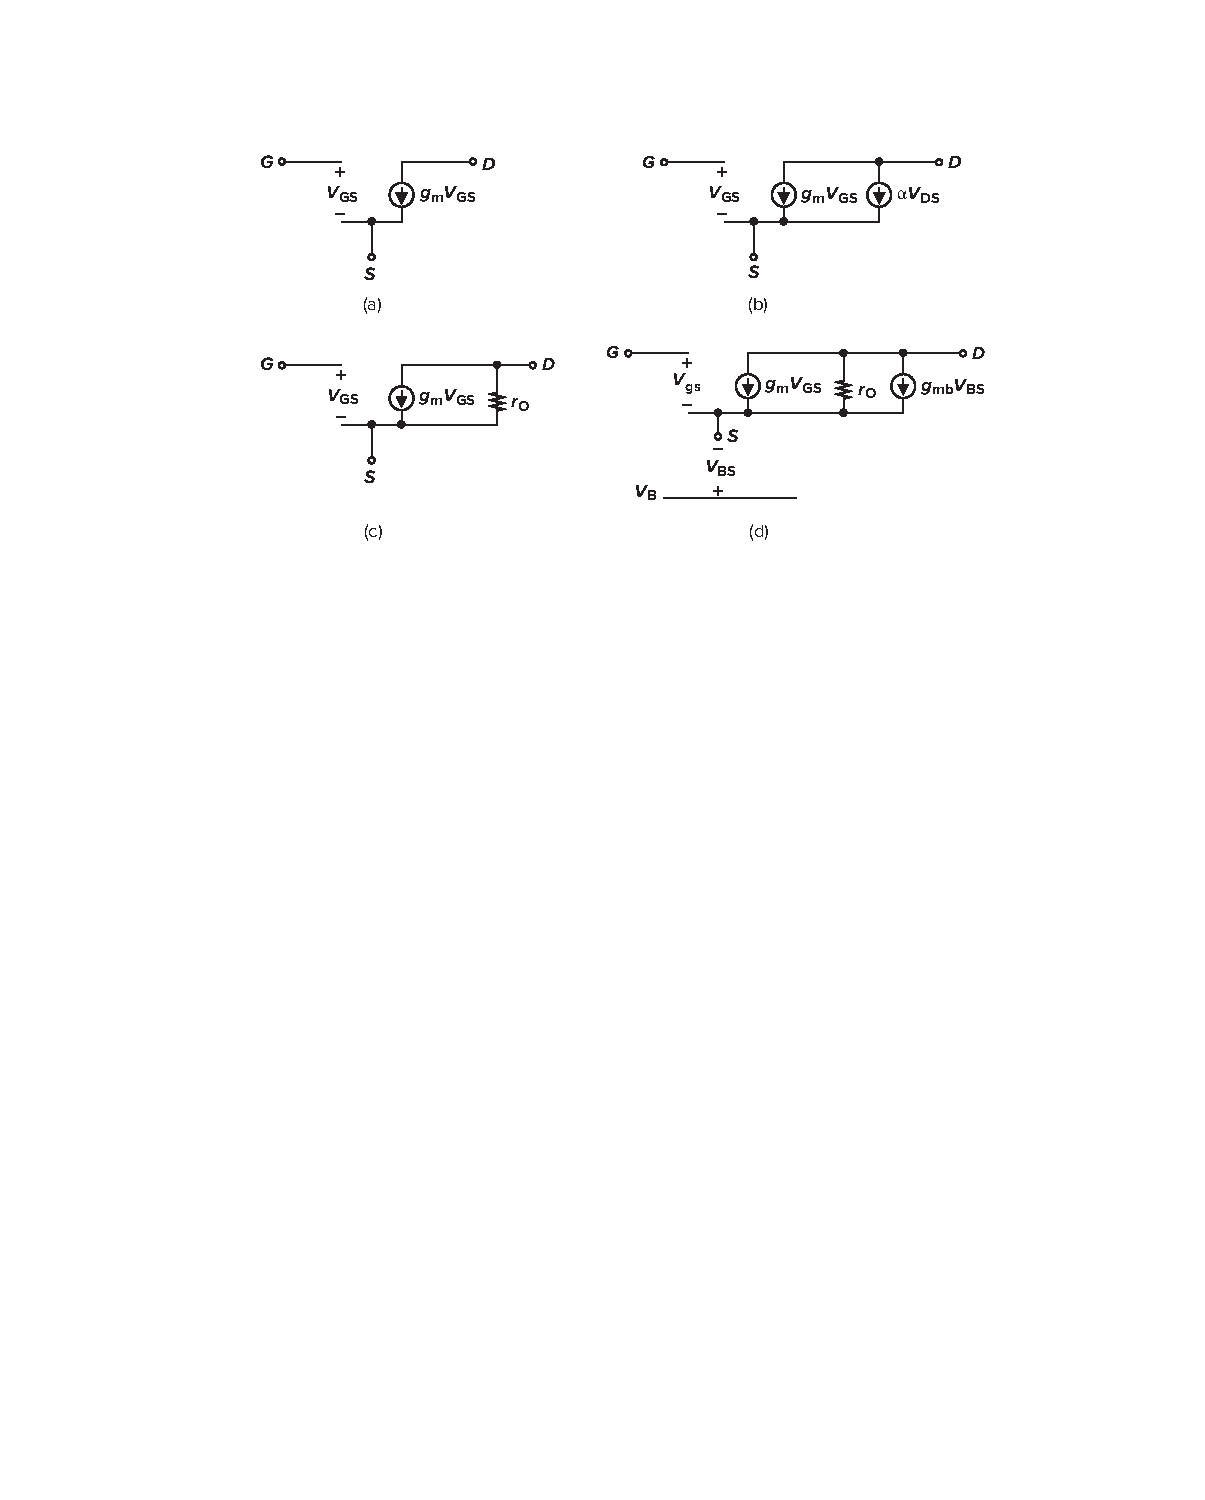
\includegraphics[width=0.7\textwidth]{MOS_small_signal_model.pdf}
    \caption{MOSFET 的小信号模型\cite{Analog-CMOS}}
    \label{fig:mosfet-small-signal-model}
\end{figure}
通常情况下我们不需要考虑体效应,在一般的分析中可以采用图 \ref{fig:mosfet-small-signal-model}(c) 所示的模型。为了简化运算,我们还可以忽略沟道长度调制效应,这样就可以使用图 \ref{fig:mosfet-small-signal-model}(a) 所示的简化模型。





\newpage
首先回顾一下一端口电路的等效。对于一个线性含源一端口电阻电路,可以进行戴维宁等效(Thevenin Equivalent)或诺顿等效(Norton Equivalent)的转换,如图 \ref{fig:thevenin-norton-equivalent} 所示。
\begin{figure}[!htb]
    \centering
    \begin{subfigure}[b]{\textwidth}
        \centering
        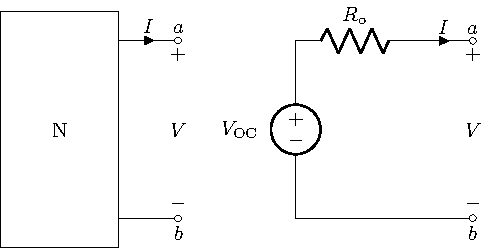
\includegraphics[]{thevenin.pdf}
        \caption{戴维宁等效}
    \end{subfigure}
    \begin{subfigure}[b]{\linewidth}
        \centering
        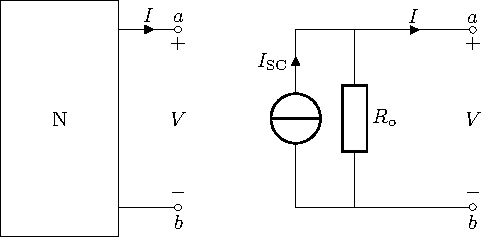
\includegraphics[]{norton.pdf}
        \caption{诺顿等效}
    \end{subfigure}
    \caption{戴维宁等效与诺顿等效}
    \label{fig:thevenin-norton-equivalent}
\end{figure}

在戴维宁等效中,$V_[OC]$为开路电压,$R_[o]$为将N内所有的独立源置零后两端钮间的等效电阻。在诺顿等效中,$I_[SC]$为短路电流,$R_[o]$同样为两端钮间的等效电阻。
它们具有关系$V_[OC] = I_[SC] \cdot R_[o]$。


% % % % % % % % % %
\part{Analog Integrated Circuits}
\chapter{Single-Stage Amplifiers}

%%%
\section{General Considerations}
从本章开始将进入模拟电路的部分。本章使用的符号如表 \ref{tab:chapter4-symbols} 所示。
\begin{table}[!htb]
    \centering
    \caption{Single-Stage Amplifiers Symbols}
    \label{tab:chapter4-symbols}
    \begin{NiceTabular}{cccc}
        \Xhline{1pt}
        \textbf{Symbol} & \textbf{Meaning} & \textbf{Unit} & \textbf{Polarity} \\ \hline
        $v_[in]$ & 输入电压(Input voltage) & $\unit{\volt}$ & $\diagdown$ \\
        $v_[out]$ & 输出电压(Output voltage) & $\unit{\volt}$ & $\diagdown$ \\
        $i_[in]$ & 输入电流(Input current) & $\unit{\ampere}$ & $\diagdown$ \\
        $i_[out]$ & 输出电流(Output current) & $\unit{\ampere}$ & $\diagdown$ \\
        $R_[in]$ & 输入电阻(Input resistance) & $\unit{\ohm}$ & + \\
        $Z_[in]$ & 输入阻抗(Input impedance) & $\unit{\ohm}$ & $\diagdown$ \\
        $R_[out]$ & 输出电阻(Output resistance) & $\unit{\ohm}$ & + \\
        $Z_[out]$ & 输出阻抗(Output impedance) & $\unit{\ohm}$ & $\diagdown$ \\
        $R_[load]/R_[L]$ & 负载电阻(Load resistance) & $\unit{\ohm}$ & + \\
        $Z_[load]/Z_[L]$ & 负载阻抗(Load impedance) & $\unit{\ohm}$ & $\diagdown$ \\
        $A_[v]$ & 电压增益(Voltage gain/Gain) & 1 & $\diagdown$ \\
        $G_[m]$ & 跨导(Transconductance) & $\unit{\siemens}$ & $\diagdown$ \\
        $g$ & 转移电导(Transfer conductance) & $\unit{\siemens}$ & $\diagdown$ \\
        \Xhline{1pt}
    \end{NiceTabular}
\end{table}

%%%%
\subsection{Equivalent of a One-Port Network}
首先回顾一下一端口电路的等效。对于一个线性含源一端口电阻电路,可以进行戴维宁等效(Thevenin Equivalent)或诺顿等效(Norton Equivalent)的转换,如图 \ref{fig:thevenin-norton-equivalent} 所示。
\begin{figure}[htp!]
    \centering
    \begin{subfigure}[b]{\textwidth}
        \centering
        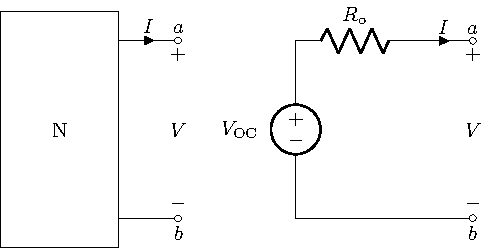
\includegraphics[]{thevenin.pdf}
        \caption{戴维宁等效}
    \end{subfigure}
    \begin{subfigure}[b]{\linewidth}
        \centering
        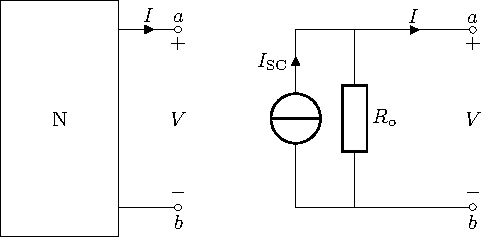
\includegraphics[]{norton.pdf}
        \caption{诺顿等效}
    \end{subfigure}
    \caption{戴维宁等效与诺顿等效}
    \label{fig:thevenin-norton-equivalent}
\end{figure}

在戴维宁等效中,$V_[OC]$为开路电压,$R_[o]$为将N内所有的独立源置零后两端钮间的等效电阻。在诺顿等效中,$I_[SC]$为短路电流,$R_[o]$同样为两端钮间的等效电阻。
它们具有关系$V_[OC] = I_[SC] \cdot R_[o]$。

%%%%
\subsection{Input and Output Impedances}
对于放大电路,我们通常会将其分为很多级,每一级都有输入和输出。为了简化,我们对其进行等效,如图 \ref{fig:input-output-impedance} 所示。
\begin{figure}[!htb]
    \centering
    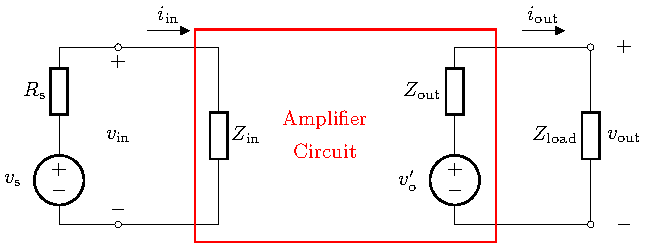
\includegraphics[]{input-output-impedance.pdf}
    \caption{放大电路示意图}
    \label{fig:input-output-impedance}
\end{figure}
需要注意,所谓的\textbf{放大电路,都是基于小信号而言的}。

\textbf{输入阻抗(Input Impedance)}$\bm{Z_{\mathrm{in}}}$是从放大电路输入端看进去的等效电阻,其值为输入端电压$v_[in]$与输入端电流$i_[in]$的比值,
\begin{equation}
    Z_[in] = \frac{v_[in]}{i_[in]}
\end{equation}
通常我们希望输入阻抗$Z_[in]$的值尽量大,这样才能使得放大电路从信号源索取的电流尽量小,降低功耗,同时使放大电路得到的输入电压$v_[in]$更接近信号源的输出电压$v_[s]$,信号电压的损失更小。

放大电路从输出端看进去,内部是一个含源一端口电路,可以等效为一个电压源与电阻串联或一个电流源与电阻并联。这个电阻就是\textbf{输出阻抗(Output Impedance)}$\bm{Z_{\mathrm{out}}}$,其值为将输入信号源置零后,输出端电压$v_[out0]$与输出端电流$i_[out0]$的比值,
\begin{equation}
    Z_[out] = \frac{v_[out0]}{i_[out0]}
\end{equation}
也可以用添加测试电流$I_[X]$或测试电压$V_[X]$的方式来测量输出阻抗。\\
通常我们希望输出阻抗$Z_[out]$的值尽量小,这样才能使得放大电路的负载能分到更大的电压,电路的带负载能力更强。

需要注意,输入阻抗是从输入端看去的,在等效电路中位于输出的位置,而输出阻抗是从输出端看去的,在等效电路中位于输入的位置。这在初学时容易记忆错误。
同时,\textcolor{red}{输入阻抗与输出阻抗之间\textbf{没有对称关系}},它们是两个不同的概念。

%%%%
\subsection{Basic Amplifier Analysis Principles}
在模拟集成电路设计中,各级放大电路一般都是基于 MOSFET 来实现的。而为了实现高的输入阻抗,一般又会采用\textbf{栅极作为输入端}。

结合 MOSFET 的小信号模型(图 \ref{fig:mosfet-small-signal-model}),我们通常使用图 \ref{fig:amplifier-equivalent-circuit} 所示的等效电路来进行分析计算。
\begin{figure}[h!tb]
    \centering
    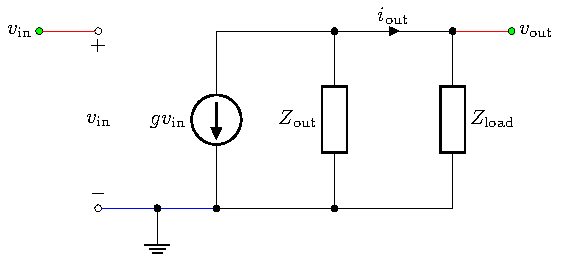
\includegraphics[]{amplifier-equivalent-circuit.pdf}
    \caption{放大电路等效电路}
    \label{fig:amplifier-equivalent-circuit}
\end{figure}
其中$g$为压控电流源(VCCS)的转移电导\footnote{转移电导$g$与放大电路的跨导$G_[m]$是两个不同的概念,转移电导是针对一个受控源而言的,而跨导是整个放大电路输出电流与输入电压的小信号比值。在JianJun Zhou的ppt中二者没有很好地区分,容易误解,在此指出。},$Z_[out]$为输出阻抗,$Z_[load]$为负载阻抗,$v_[in]$为输入电压,$v_[out]$为输出电压。

注意图 \ref{fig:amplifier-equivalent-circuit} 中的输入端的等效电源是一个受控源而不是独立源,但这并不是误用诺顿等效。这个受控源的电流是$g v_[in]$,转移电导$g$是由电路的静态工作点(大信号)决定的,而输入电压$v_[in]$是由上一级电路决定的,因此这个受控源的电流实际不受这一级小信号放大电路本身的影响,相对于当前的小信号电路是独立的,是一个“独立源”。

将单级放大电路简化为图 \ref{fig:amplifier-equivalent-circuit} 所示的形式后,容易看出其\textbf{增益(Gain)$A_[v]$}为
\begin{equation}
    A_[v] = \frac{v_[out]}{v_[in]} = -g (Z_[out] // Z_[load])
    \label{eq:amplifier-gain}
\end{equation}
式 \ref{eq:amplifier-gain} 非常重要,在后续的分析中会经常用到。有时我们在计算时会忽略负号,仅考虑增益的绝对值(电压放大的倍数)。

这里说明几个初学小信号电路图时令人困惑的问题(有些大信号电路图也有这些问题)。
\begin{itemize}
    \item \textbf{小信号输入和输出都是相对于地的}。小信号输入电压$v_[in]$和输出电压$v_[out]$都是相对于地的电压。很多时候在图中输入输出电压只接入了一个端钮,例如图 \ref{fig:amplifier-equivalent-circuit} 中的绿色端钮。我们应该知道另一个端钮是没有画出的接地点。

    \item \textbf{有些导线中是没有电流的,它只表示两个节点的电位相等}。很多时候,为了表示多个节点都接地,我们会用导线将这些节点相连避免在图中绘制多个接地点。这些导线中是没有电流的,它只表示两个节点的电位相等,在分析电流时可直接将其忽略。图 \ref{fig:amplifier-equivalent-circuit} 中的蓝色导线就是一个例子。

    \item \textbf{有些端钮是悬空的,只代表一个电压探针}。有些时候,为了简化图形,我们会将某些端钮悬空,引出一条悬空导线并给出一个电压值标签,代表一个电压探针。例如图 \ref{fig:amplifier-equivalent-circuit} 中的$v_[out]$。与探针相连的导线中是没有电流的,只是为了作图的方便引出一条导线。图 \ref{fig:amplifier-equivalent-circuit} 中的红色导线中是没有电流的。但需要注意,并不是所有这样的端钮都代表探针,例如一些大信号电路图中的$V_[DD]$就不是探针,它是一个电源,与其相连的导线中是有电流的。
\end{itemize}
这些特殊情况并不会在图中标出,需要我们自己去判断理解。

%%%%
\subsection{``Common'' What?}
在分析放大电路时,我们经常会遇到“共X放大电路”(Common Xxx)的概念,例如“共源放大电路”(Common Source Amplifier,CS Amplifier),“共栅放大电路”(Common Gate Amplifier,CG Amplifier),“共漏放大电路”(Common Drain Amplifier,CD Amplifier)等等。这里的“共”到底是什么意思呢?


% % % % % % % % % %
\part{Digital Integrated Circuits}

\bookmarksetupnext{level=-1}
\appendix
\chapter{Appx Title}
Nothing here yet.


% % % % % % % % % %
\backmatter
\bookmarksetupnext{level=-1}
% 使用 bibLaTeX 制作书目
\nocite{*}	% 列出所有参考文献, 即使未在正文中引用
\printbibliography[heading=bibintoc]

% 图, 表索引. 可有可无.
\bookmarksetupnext{level=-1}
\listoffigures
\bookmarksetupnext{level=-1}
\listoftables

% 制作索引 (用 imakeidx 的功能可以制作多份)
{\footnotesize
	\indexprologue{中文术语按汉语拼音排序.}
	\printindex}

\end{document}
